\begin{refsection}[research/tsubokura/group.bib]
\nocite{*}
\chapter{Complex Phenomena Unified Simulation Research Team}

\section{Members}

\begin{itemize}
  \item[] Makoto Tsubokura (Team Leader)
  \item[] Keiji Onishi (Postdoctoral Researcher)
  \item[] Chung-gang Li (Postdoctoral Researcher)
  \item[] Leif Niclas Jansson (Postdoctoral Researcher)
  \item[] Rahul Bale (Postdoctoral Researcher)
  \item[] Tetsuro Tamura (Visiting Researcher)
  \item[] Ryoichi Kurose (Visiting Researcher)
  \item[] Gakuji Nagai (Visiting Researcher)
  \item[] Kei Akasaka (Visiting Researcher)
  \end{itemize}

\section{Research Activities}

The objective of our research team is to propose a unified simulation method of solving multiple partial differential equations by developing common fundamental techniques such as the effective algorithms of multi-scale phenomena or the simulation modeling for effective utilization of the massively parallel computer architecture. The target of the unified simulation is supposed to be complex and combined phenomena observed in manufacturing processes in industrial circles and our final goal is to contribute to enhance Japanese technological capabilities and industrial process innovation through the high-performance computing simulation.

Most of the complex flow phenomena observed in manufacturing processes are relating to or coupled with other physical or chemical phenomenon such as turbulence diffusion, structure deformation, heat transfer, electromagnetic field or chemical reaction. While computer simulations are rapidly spreading in industry as useful engineering tools, their limitations to such coupled phenomena have come to realize recently. This is because of the fact that each simulation method has been optimized to a specific phenomenon and once two or more solvers of different phenomena are coupled for such a complicated target, its computational performance is seriously degraded. This is especially true when we utilize a high-performance computer such as K-computer. In such a situation, in addition to the fundamental difficulty of treating different time or spatial scales, interpolation of physical quantities like pressure or velocity at the interface of two different phenomena requires additional computer costs and communications among processor cores. Different mesh topology and hence data structures among each simulation and treatment of different time or spatial scales also deteriorate single processor performance. We understand that one of the keys to solve these problems is to adopt unified structured mesh and data structure among multiple simulations for coupled phenomena. As a candidate of unified data structure for complicated and coupled phenomena, we focused on the building-cube method (BCM) proposed by Nakahashi[1].

\begin{flushleft}
[1]K. Nakahashi, High-Density Mesh Flow Computations with Pre-/Post-Data Compressions, Proc. AIAA 17th CFD Conference (2005) AIAA 2005-4876
\end{flushleft}


\section{Research Results and Achievements}
\subsection{Development of a unified framework for large-scale multiphysics problems}
Based on the Building Cube Method (BCM), we have developed a unified solver framework CUBE (Complex Unified Building cubE) for solving large-scale multphysics problems. The framework has a modular design where CUBE provides a core library containing kernel functionalities e.g. a mesh, flow fields and I/O routines. Solvers are then developed on top of the kernel by connecting necessary kernel modules together, forming a solver pipeline, describing the necessary steps to solve a particular problem.

{\bf Load balancing} is an essential component in today's large scale multiphysics simulations, and with an ever increasing amount of parallelism in modern computer architecture it is essential to reduce even the slightest workload imbalance. An imbalance could severely impact an application's scalability. Traditionally, load balancing is seen as a static problem, closely related to the fundamental problem of parallel computing, namely data decomposition. For a CFD simulation based on BCM, since each cubes contains the same amount of cells the goal is to evenly distribute the cubes among the available cores. However, such a decomposition assumes that the workload for each cube is uniform. For most cubes this is true, but for cubes which contain immersed bodies, combustion, chemical reactions, etc. the workload is slightly higher, which implies a workload imbalance. Therefore, to retain good scalability a load balancing method that balances the workload not only considering the BCM mesh, but also the additional workload from the immersed body, chemical reactions, etc., was developed.

\begin{figure}[h!]
\centering
  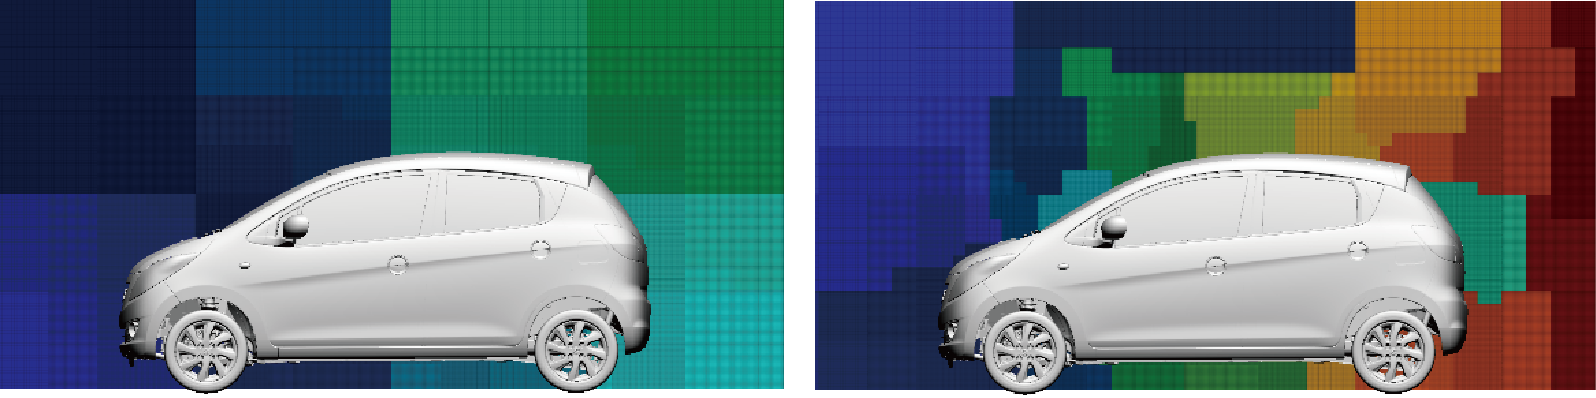
\includegraphics[height=3cm]
  {research/tsubokura/fig1.png}
  \caption{An example of load balancing with respect to the cost of evaluating the immersed geometry and the cost of computing the fluid cells, colored by MPI rank.}
  \locallabel{fig:sample-label1}
\end{figure}


To evaluate the performance of the load balancer, we used CUBE to solve two different incompressible flow problems (full vehicle and a landing gear model) on the K computer. And, the total execution time for performing a fixed number of time steps for both an unbalanced (no load balancing) and a balanced case (using load balancing) on various numbers of cores are compared (Figure~\localref{fig2}).

\begin{figure}[h!]
\centering
  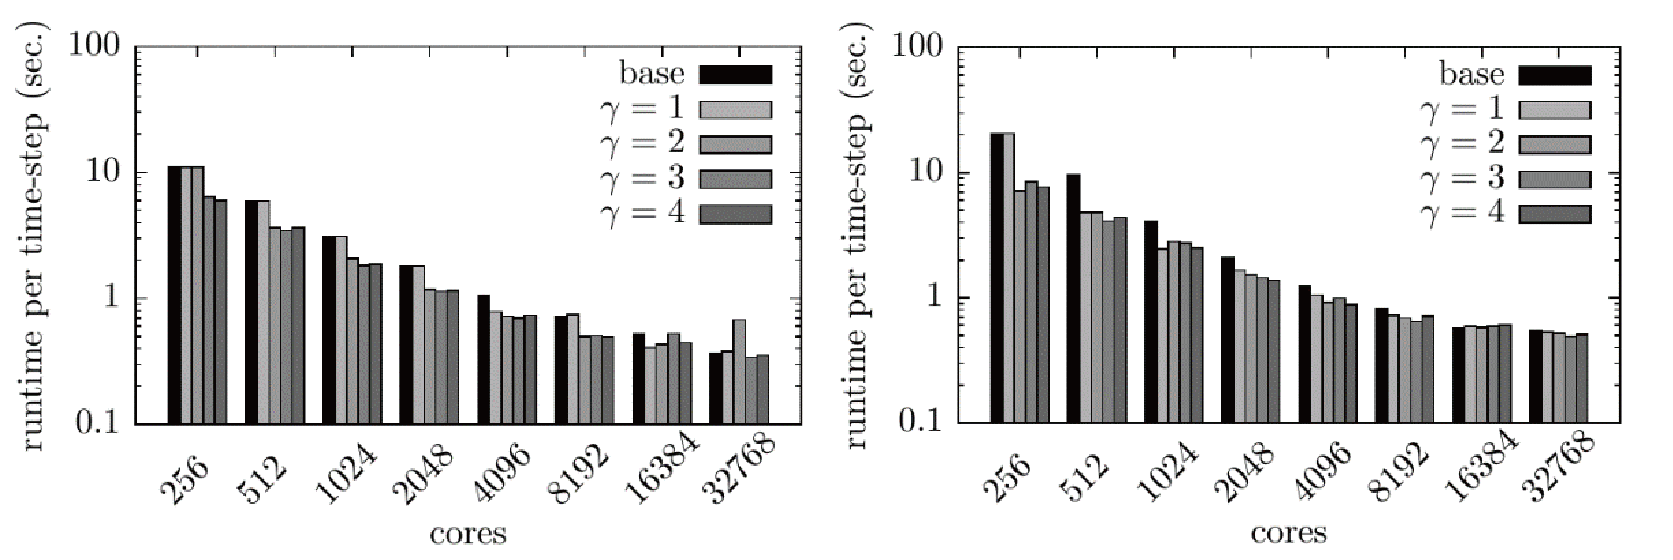
\includegraphics[height=5cm]
  {research/tsubokura/fig2.png}
  \caption{Comparison of  runtime per time-step for balanced and un balanced cases for the landing gear model (left) and the vehicle model (right)}
  \locallabel{fig2}
\end{figure}

\subsection{Development of a very large scale incompressible flow solver with a hierarchical grid system}
The CUBE, name of our software framework, has been developed by conjunction with incompressible flow code which developed to realize the analysis in a real development process of industrial field on the massively parallel environment, including pre- and post-processing.

{\bf Industrial collaboration, MAZDA}: We have utilized it for the complexed geometrical analysis using dirty CAD data received from automotive company. In last year, we have conducted basic aerodynamics validation using the vehicle geometry of MAZDA Motor Corporation. The conclusion was we need to improve an accuracy of drag force prediction. In this year, we have improved it conducting method survey of interpolation technique onto surface/volume, and the fundamental investigation of approximate domain method on immersed boundary (IB). The difficulty was came from the uncertainty of front/back face of complicated geometry because the interpolation caused huge error if the search of face orientation has been missed. It was highly depends on the complexity of geometry and grid resolution. The method which is drawn by the analogy of Poisson solver providing a front/back face information based on flow solution has been developed. Then we could successfully get a reasonable absolute drag value (about 2\% error), and drag delta between 2 different aerodynamic configurations. At the same time, we could successfully reproduce the characteristic total pressure flow field comparing to wind-tunnel measurement data.


\begin{figure}[h!]
\centering
  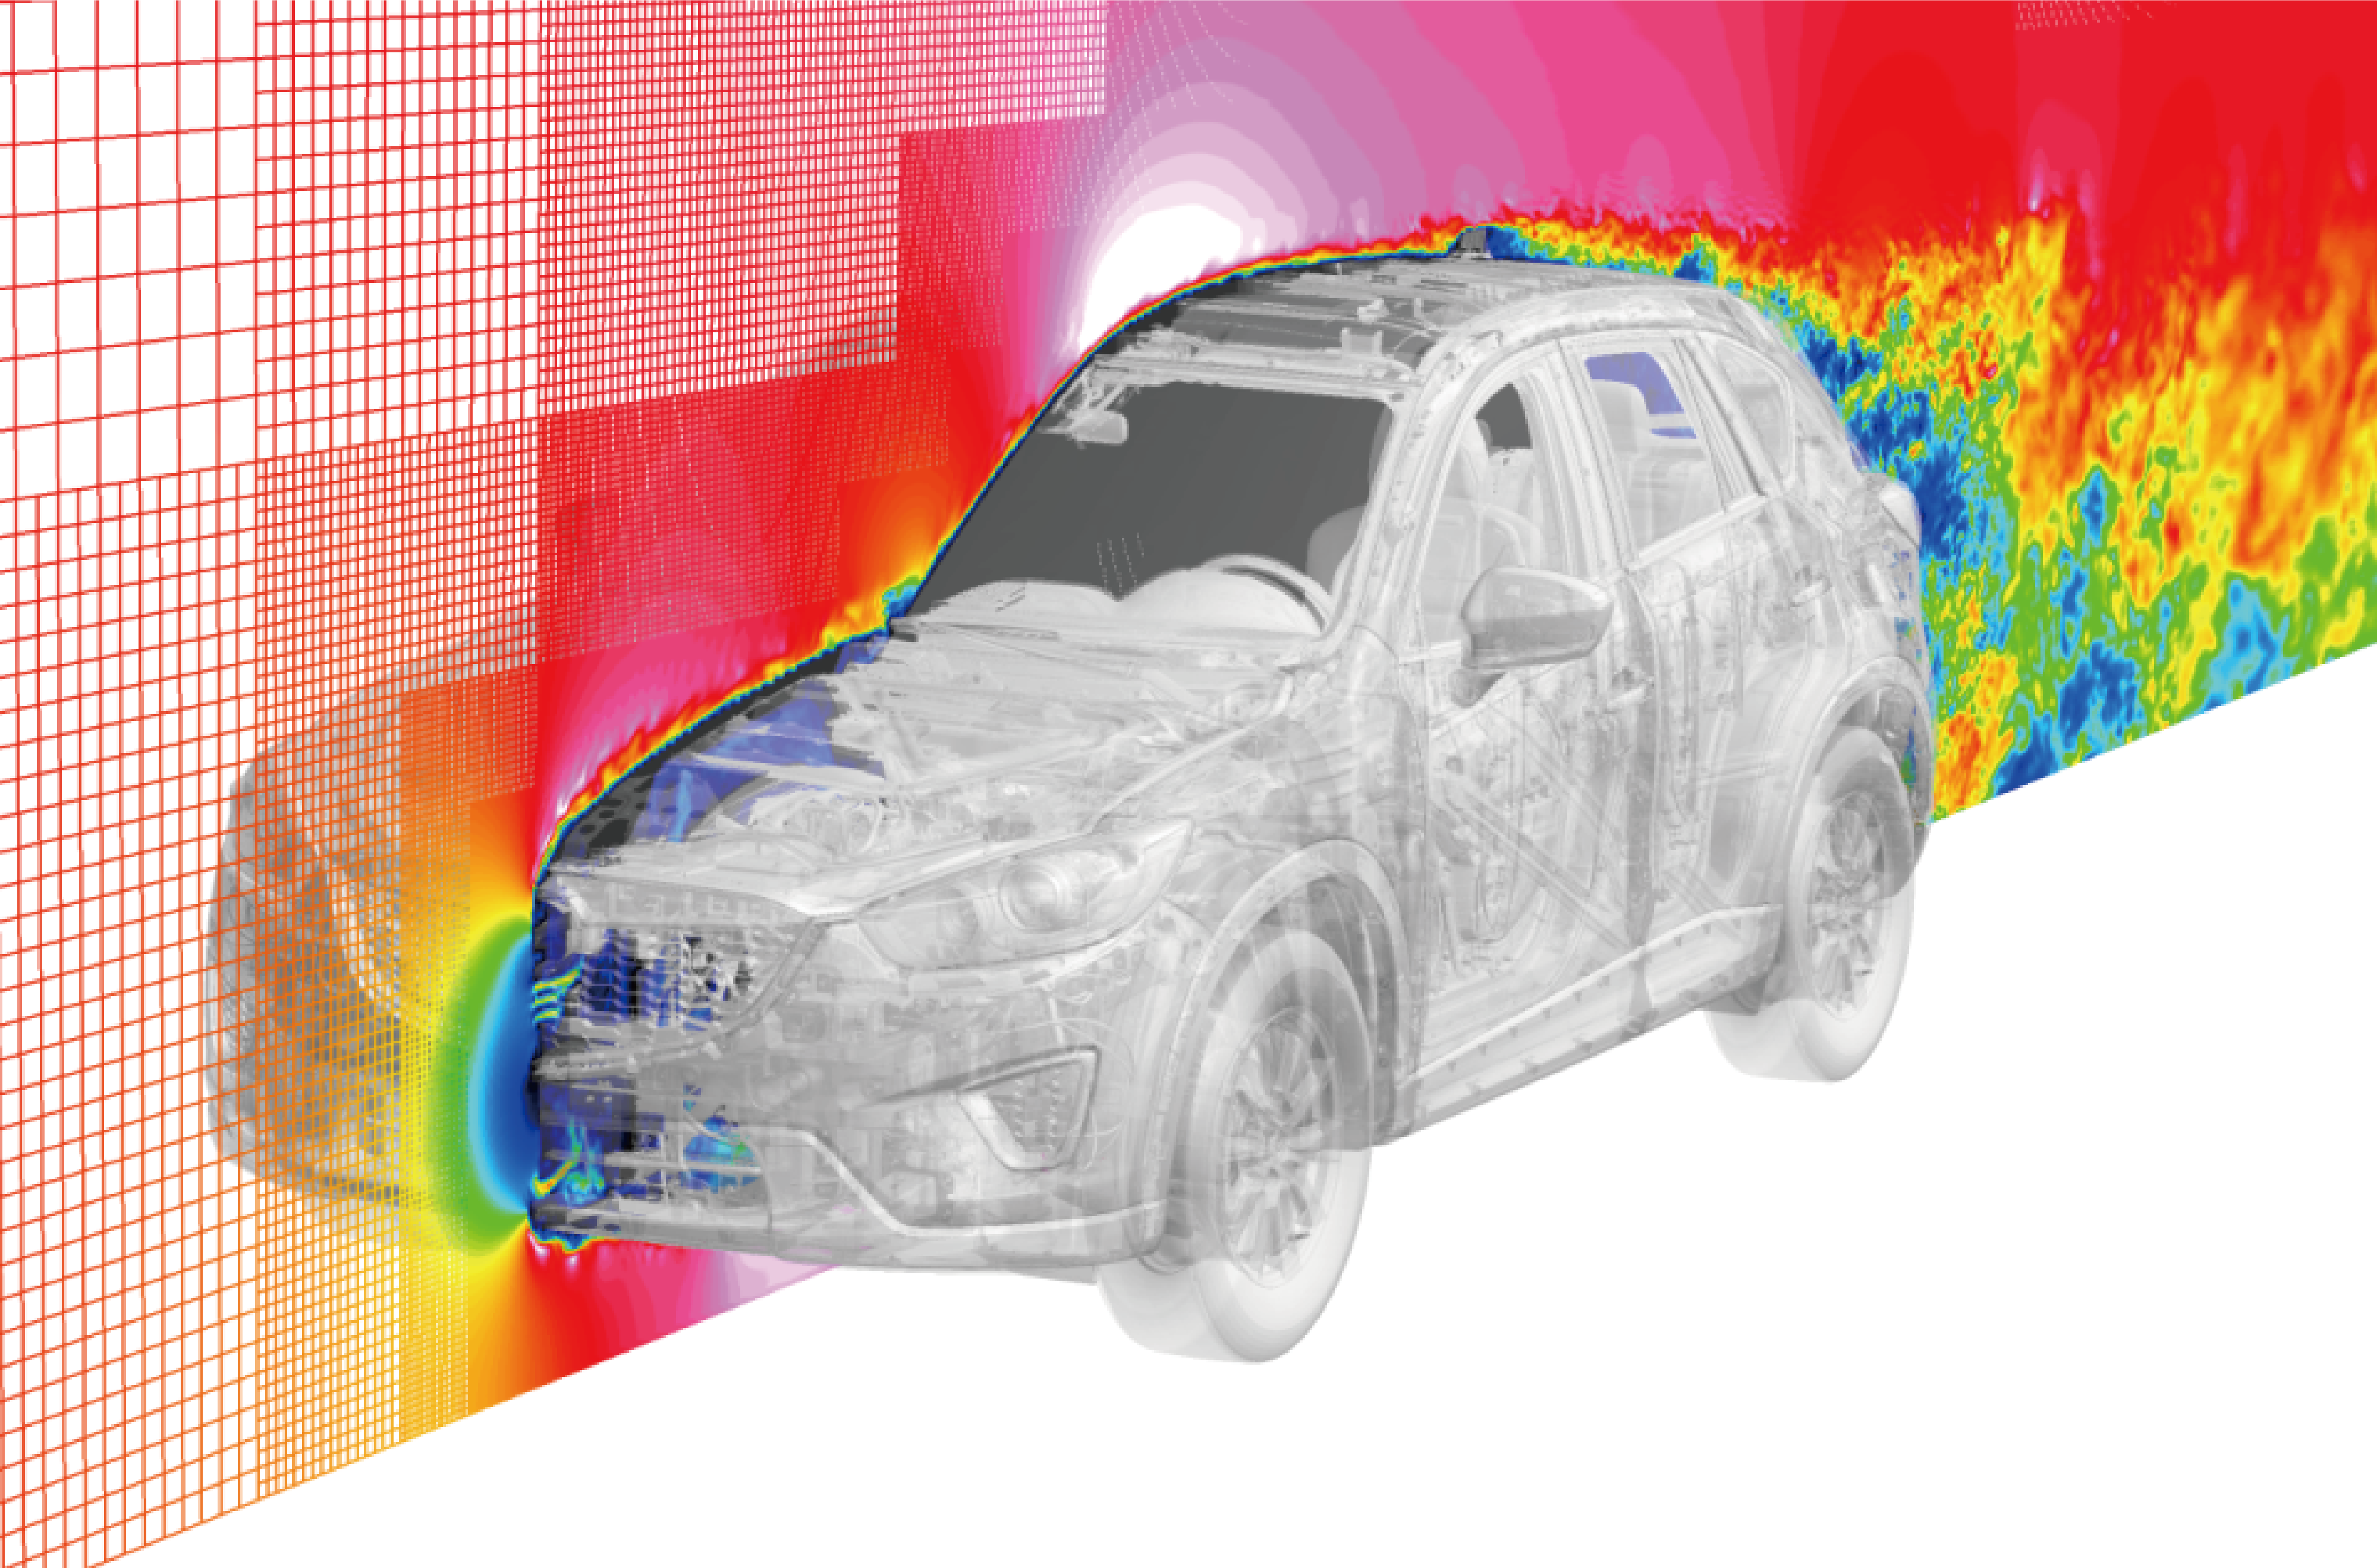
\includegraphics[height=5cm]
  {research/tsubokura/fig3.png}
  \caption{Overview of computational grid and flow field (MAZDA Motor Company).}
  \locallabel{fig3}
\end{figure}

\begin{table}[hbtp]
  \caption{predicted drag on 2 configurations normalized by experimental base case.}
  \label{table1}
  \centering
  \begin{tabular}{lcr}
    \hline
    $C_d$  & Exp.  &  Sim.  \\
    \hline
    Base  & 1.000  & 1.021 \\
    Aero  & 1.011   & 1.043 \\
    $\Delta C_d$  & 1.15\%  & 1.46\% \\
    \hline
  \end{tabular}
\end{table}

{\bf Industrial collaboration, SUZUKI}: The usability on the practical use of industrial application has been evaluated by discussing with professional engineers of automobile company. we have corroborated with SUZUKI MOTOR CORPORATION to do this work. We have provided CUBE to them with simple documents and training, and they have evaluated by their own way, and gave us their feedback report. The geometry preparation time has been accelerated from 35 hours using commercial software to 2 hours using CUBE framework, based on dirty CAD data. The estimated drag coefficient between 2 configuration had better agreement with measurement than commercial code. It shows CUBE is already ready for usage in the actual design process in term of the usability, human-cost, accuracy, and turn-around time. But, they had a strong request to improve calculation time because their process has a limitation to finish each job within 1 night whereas our method requires 2 or 3 days. To say more, their method is based on Reynold averaged approach based on strong turbulence model which is known to have relatively large error, our method is based on the pure transient approach which generally requires 10 times larger calculation resource comparing to RANS. After the discussion, we have agreed to improve it in near future because it is very important to know the true needs on the field of industrial engineering. As the first step of that, we have developed a new function to enable us to use local refinement grids in the grid generation software. It can reduce the calculation load about from 1/5 to 1/10 for the vehicle case, to accelerate the solution. And the implementation and testing of the local refinement functionality for IB has been started in this year. We thinks it also can lead to the enhancement of effective multi-grid method (MG), or adaptive mesh refinement method (AMR) in the future development scope.

Both of MAZDA and SUZUKI could decide to promote the results inside their organization, and continue the current research activity using our software in FY2016 by submitting the application and accepted the industrial use project on K-computer.

\begin{figure}[h!]
\centering
  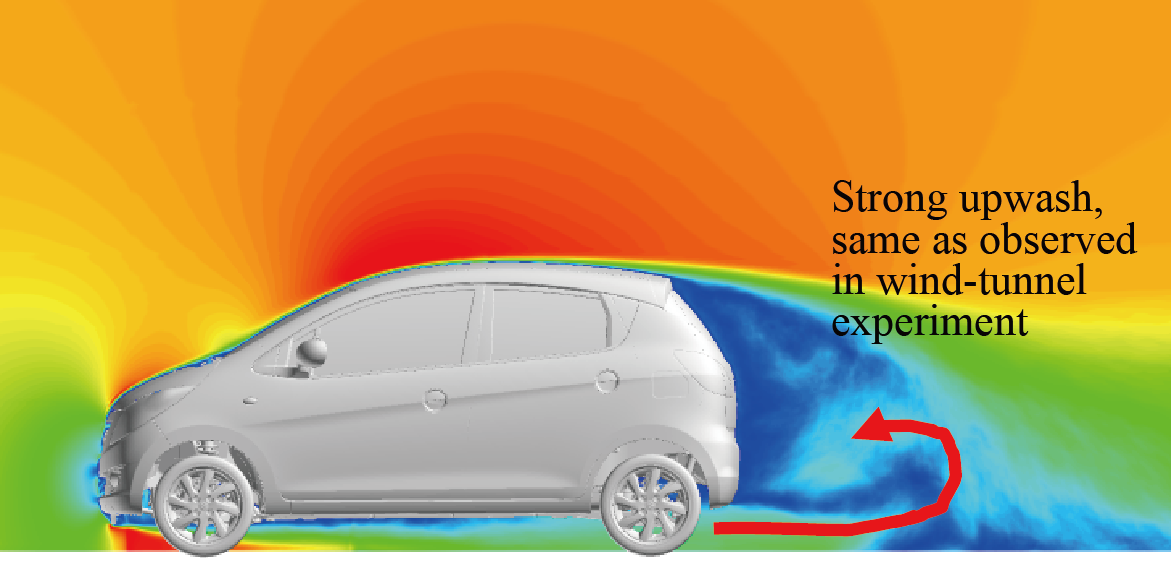
\includegraphics[height=5cm]
  {research/tsubokura/fig4.png}
  \caption{Overview of characteristic flow field (SUZUKI MOTOR CORPORATION).}
  \locallabel{fig4}
\end{figure}

\begin{table}[hbtp]
  \caption{predicted drag on 2 configurations normalized by experimental base case.}
  \label{table2}
  \centering
  \begin{tabular}{lcr}
    \hline
    Condition  & CUBE  &  Commercial Code A  \\
    \hline
Finest grid size	& 2.0 [mm]  &	2.0 [mm] (layer 0.04[mm]) \\
Num. of cells &	400 million & 53 million \\
Fluid Configuration  &	LES (Standard Smagorinsky) & DES (SST k-$\omega$) \\
Num. of timesteps & 145,000 & 4,000 \\
CAD prepare & 8 hours & 8 hours \\
Pre processing time & 2 hours	& 34.5 hours \\
Parallel num. &	4,096 cores (K-computer)  & 512 cores (Intel Xeon) \\
Flow computation time & 258 hours & 8 hours \\
Post processing time & 1.5 hours & 1.2 hours \\
Error of Cd prediction & Applx. 10\% & Applx. 11-16\% \\
Error of $\Delta C_d$  prediction  & 8\%  & 12\% \\
    \hline
  \end{tabular}
\end{table}


{\bf Wind HPC consortium}: At a research activity on Wind-HPC consortium which is organized by Tokyo Institute of Technology and several Japanese major construction companies, the detailed turbulence characteristics on wind canopy of actual urban area geometry that has housings, buildings, vegetation, and street, and so on, has been investigated. And, the academic case validation using square cylinder has been conducted. The results shows reasonable accuracy, so both of results has been published in the paper of architecture design. This research will continue on the FLAGSHIP 2020 project of priority $\sharp$ 4 regarding wind environment evaluation for building construction on severe climate condition through next years.


\begin{figure}[h!]
\centering
  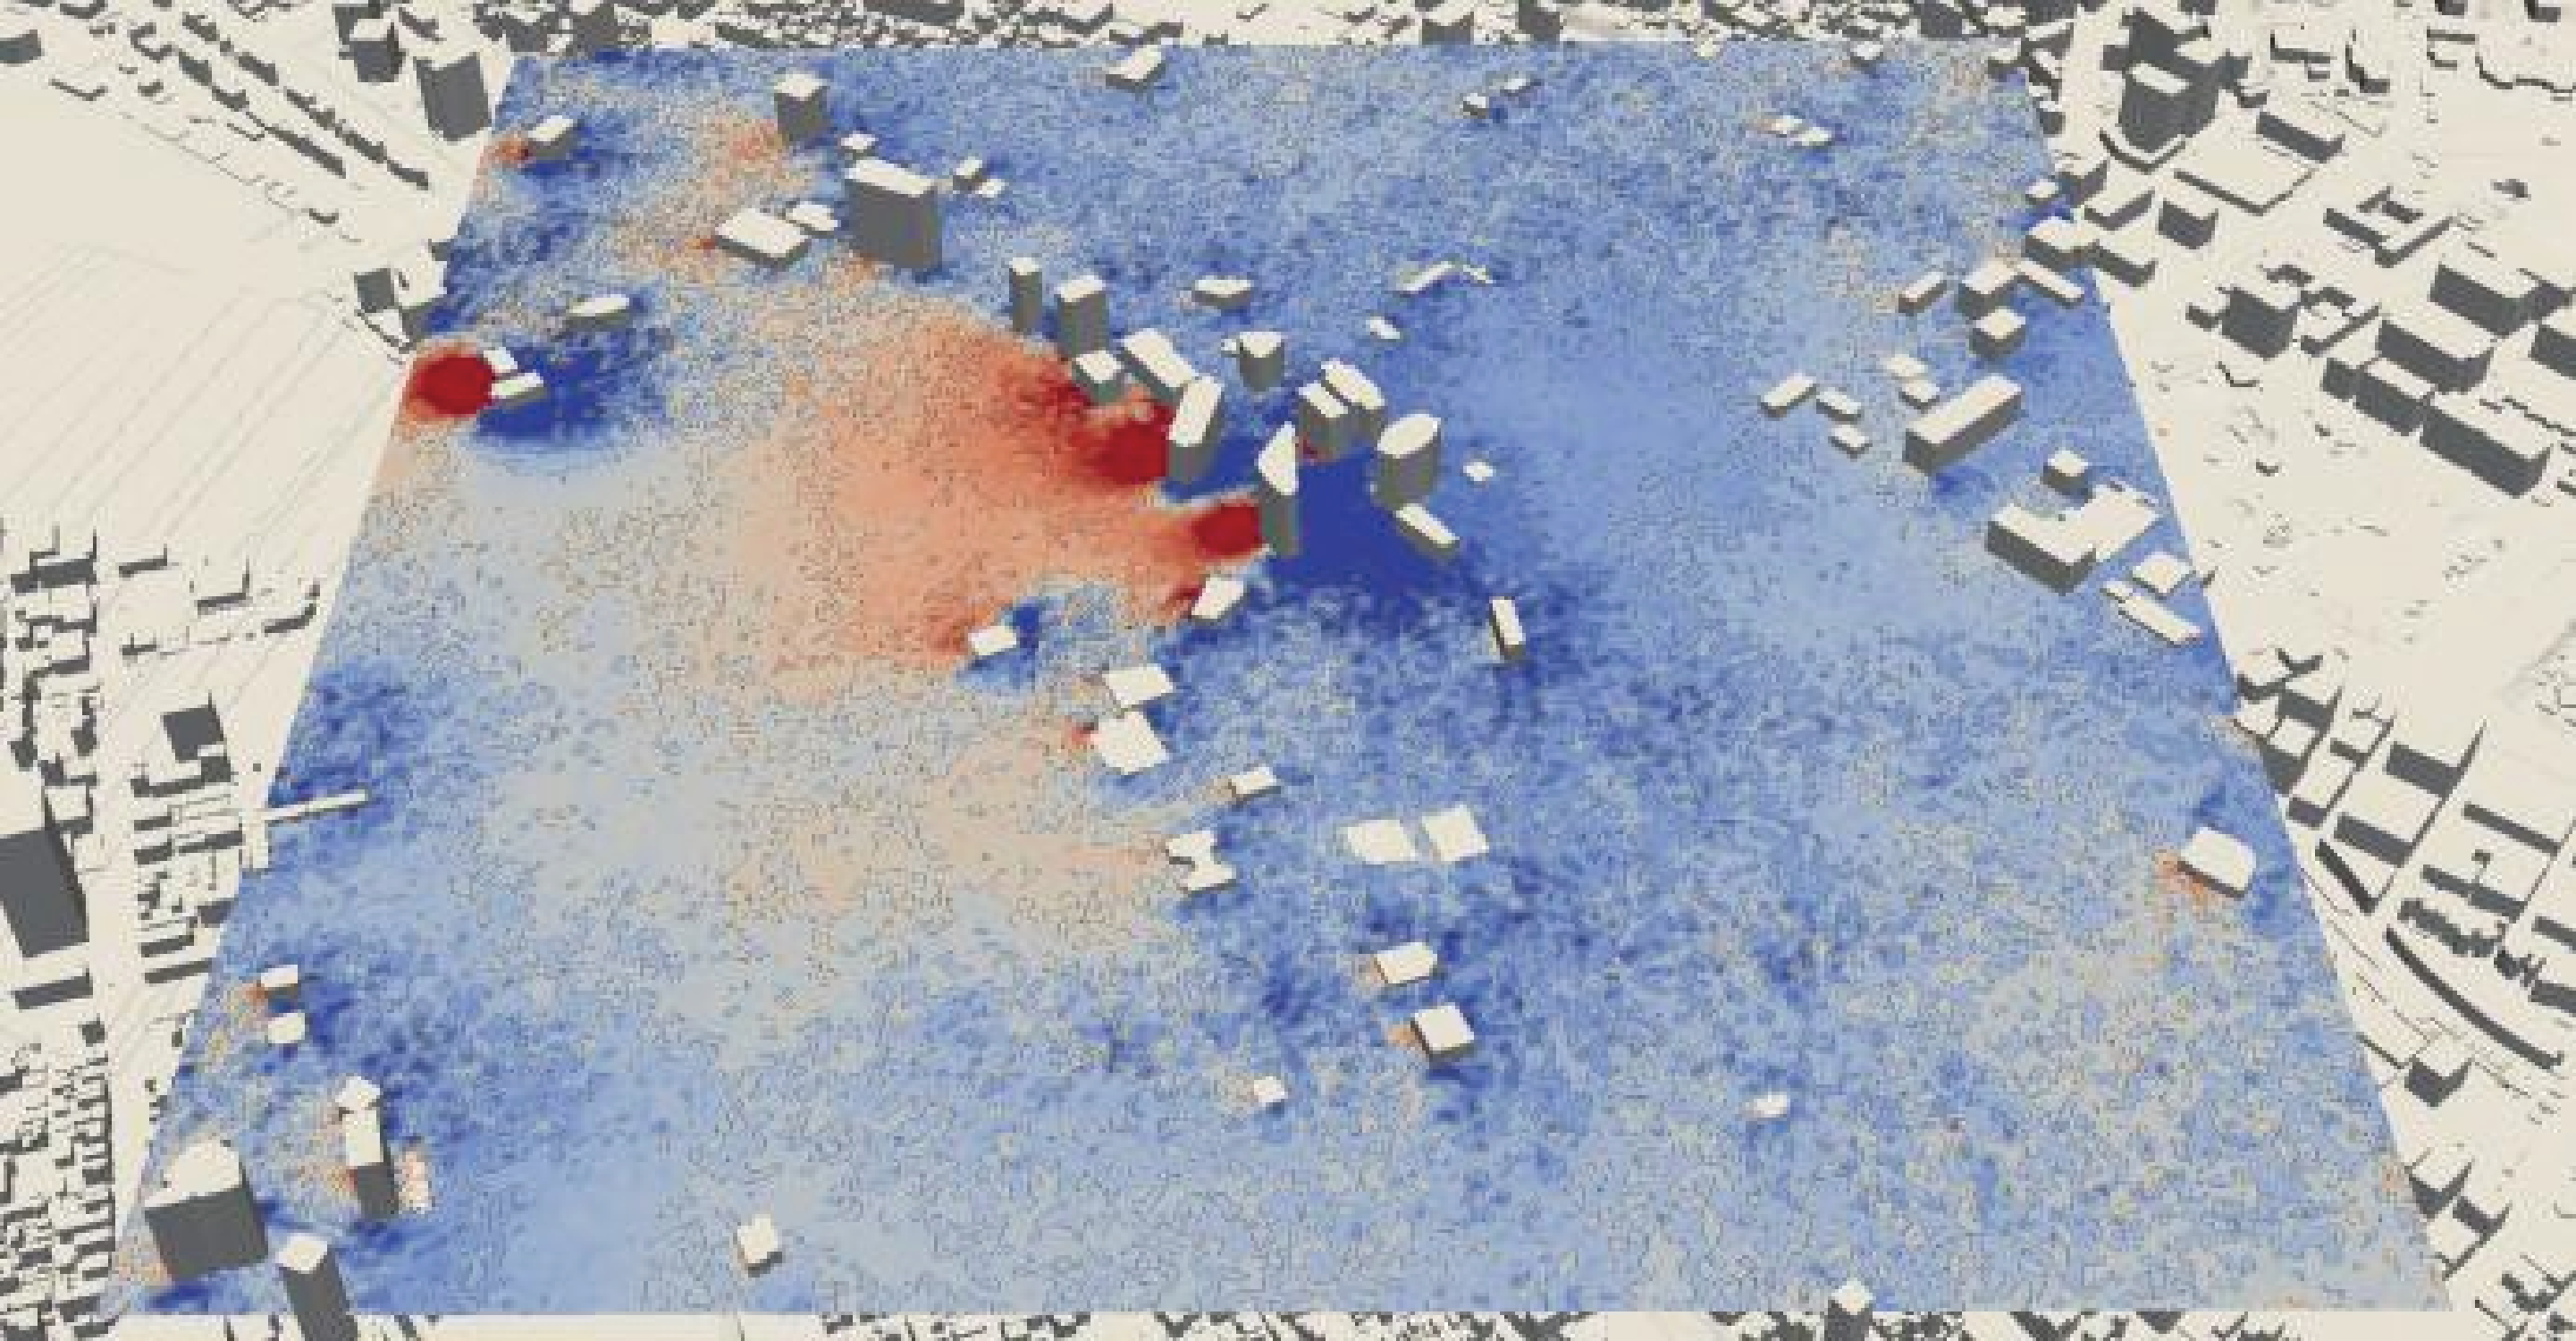
\includegraphics[height=3cm]
  {research/tsubokura/fig5_1.png}
  \caption{Pressure field in Shiodome area(50m Height)}
  \locallabel{fig51}
\end{figure}

\begin{figure}[h!]
\centering
  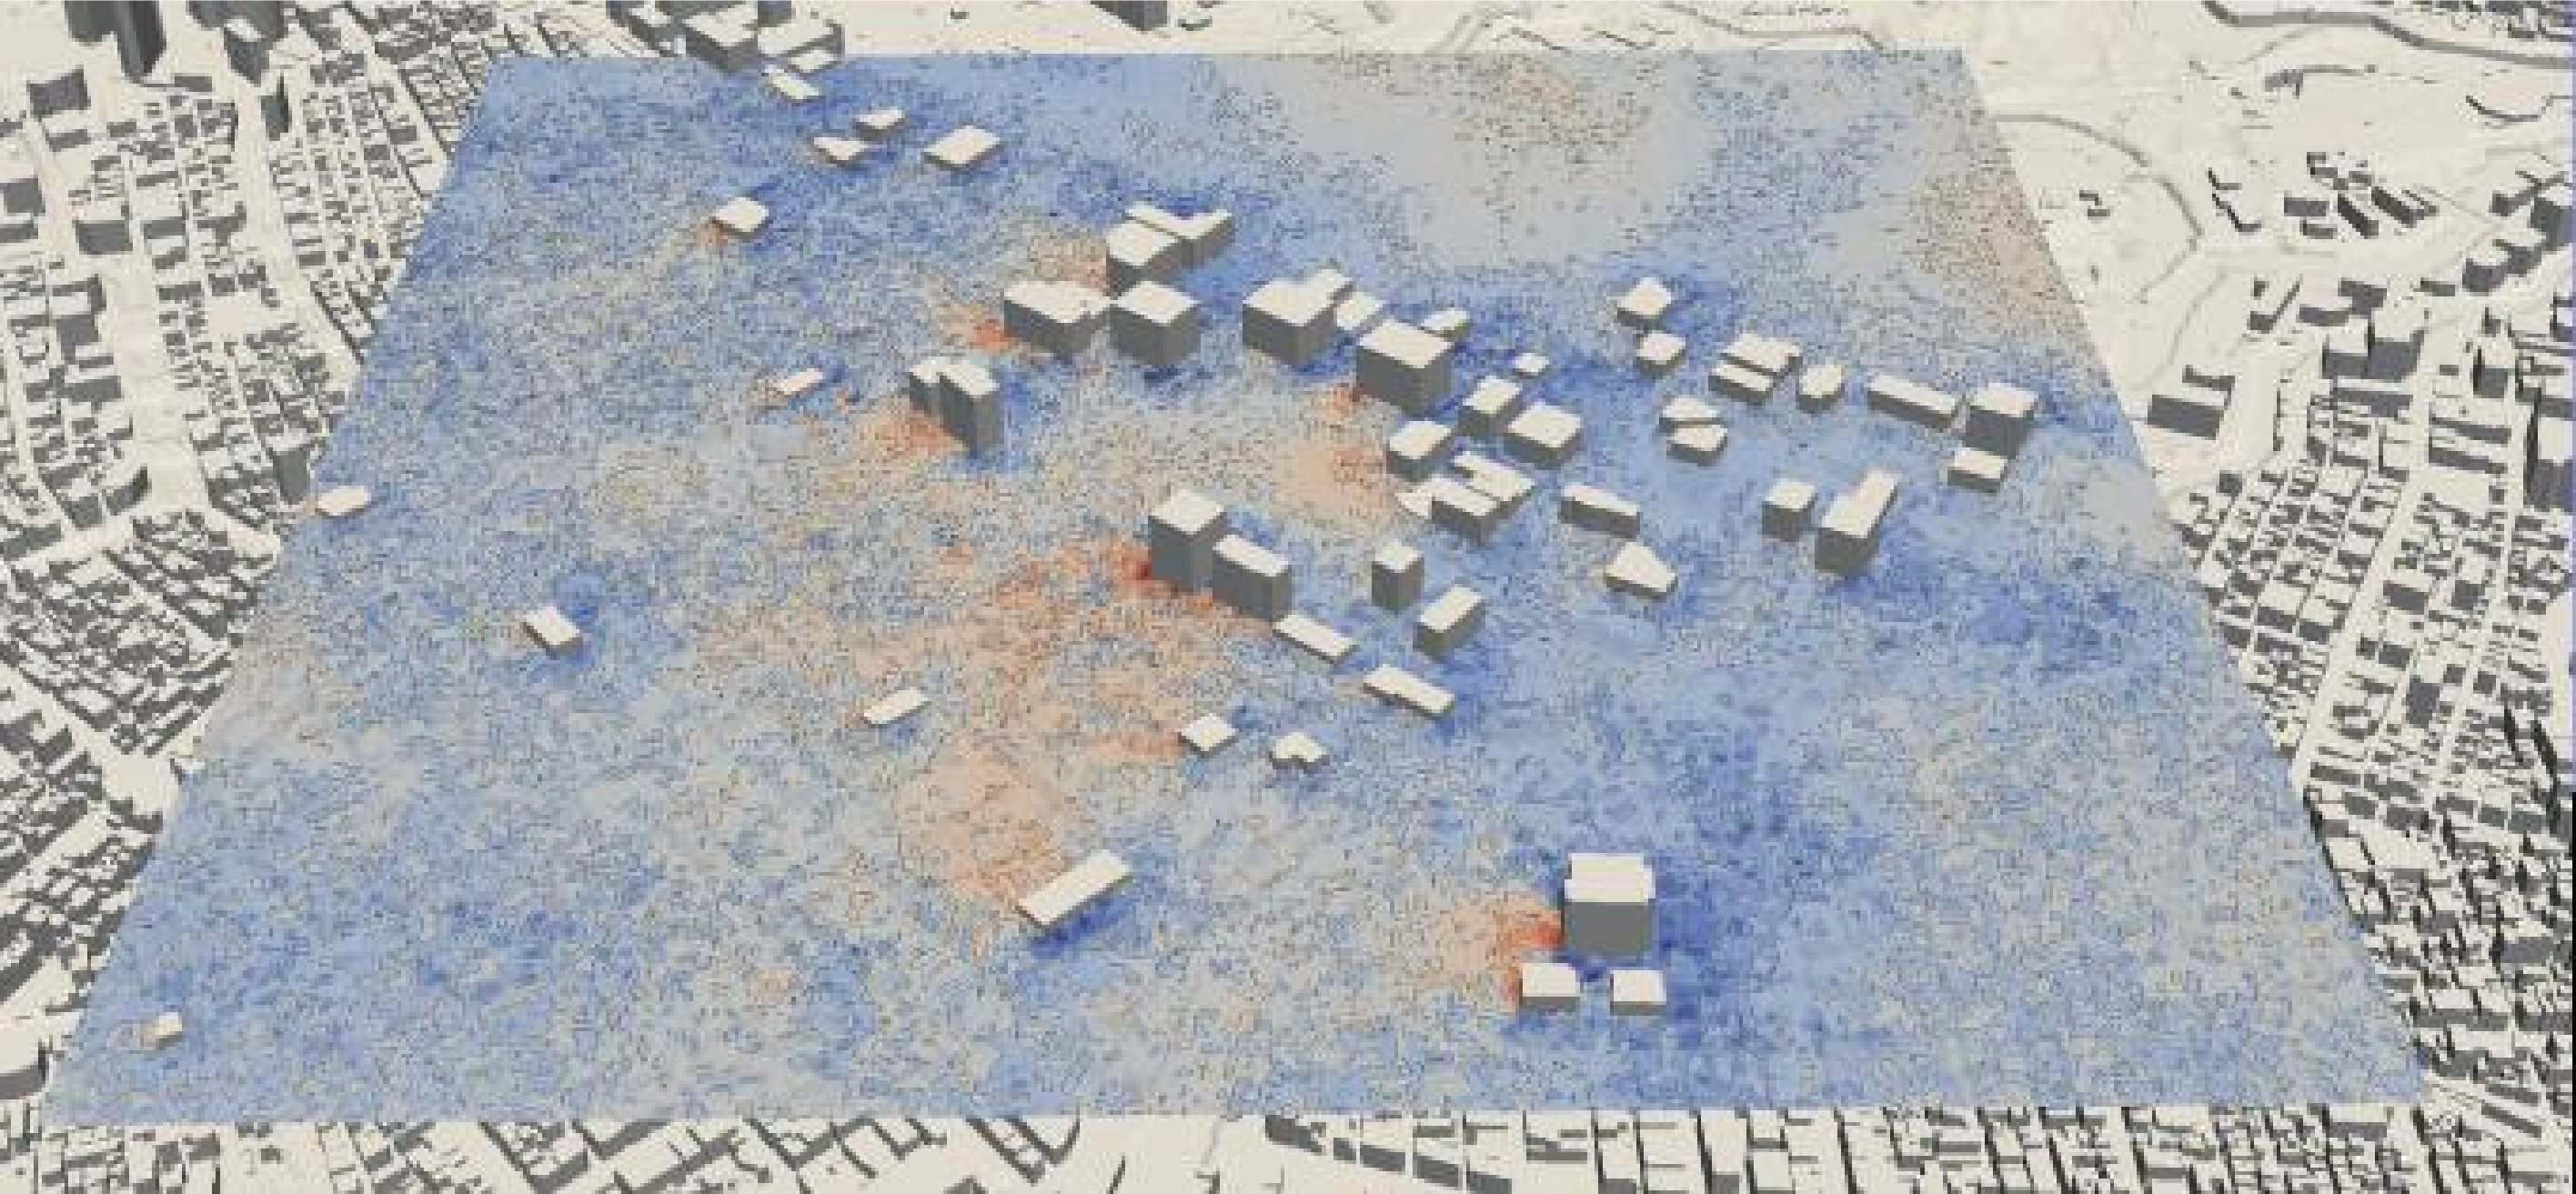
\includegraphics[height=3cm]
  {research/tsubokura/fig5_3.png}
  \caption{Pressure field in Marunouchi area(50m Height)}
  \locallabel{fig53}
\end{figure}

\begin{figure}[h!]
\centering
  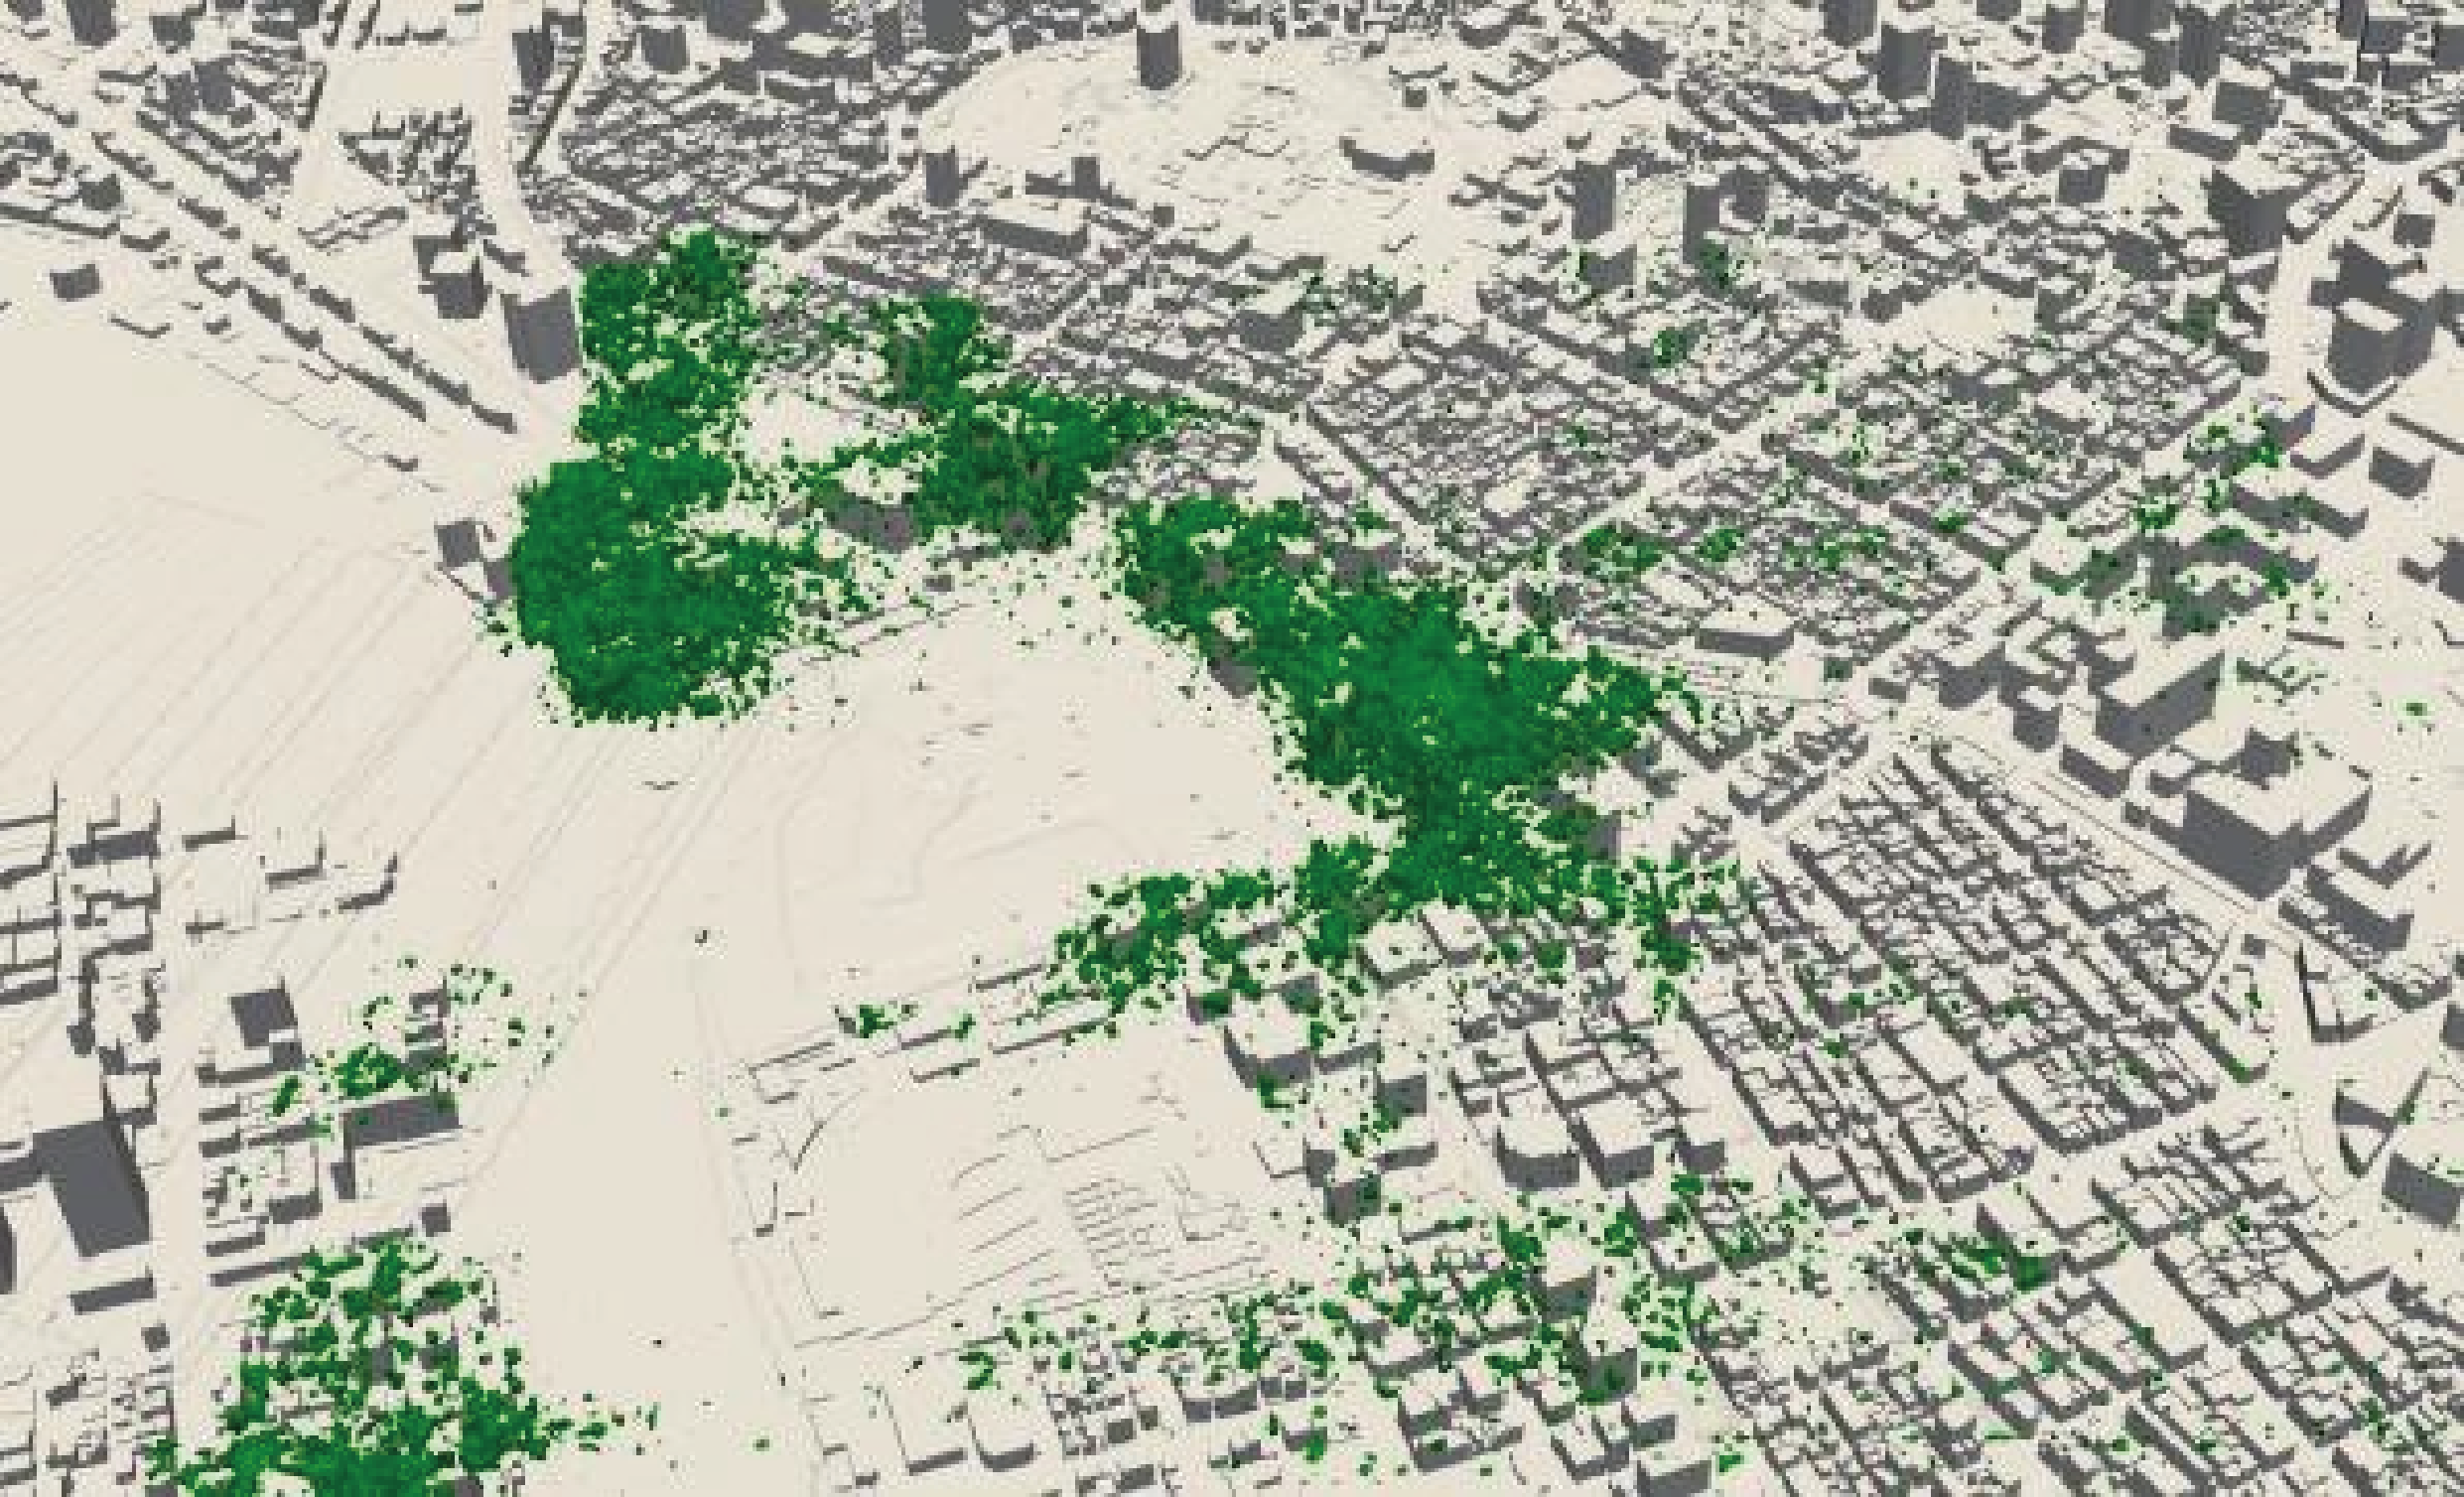
\includegraphics[height=3cm]
  {research/tsubokura/fig5_2.png}
  \caption{Q-criterion (Q=0.0015) in Shiodome area}
  \locallabel{fig52}
\end{figure}

\begin{figure}[h!]
\centering
  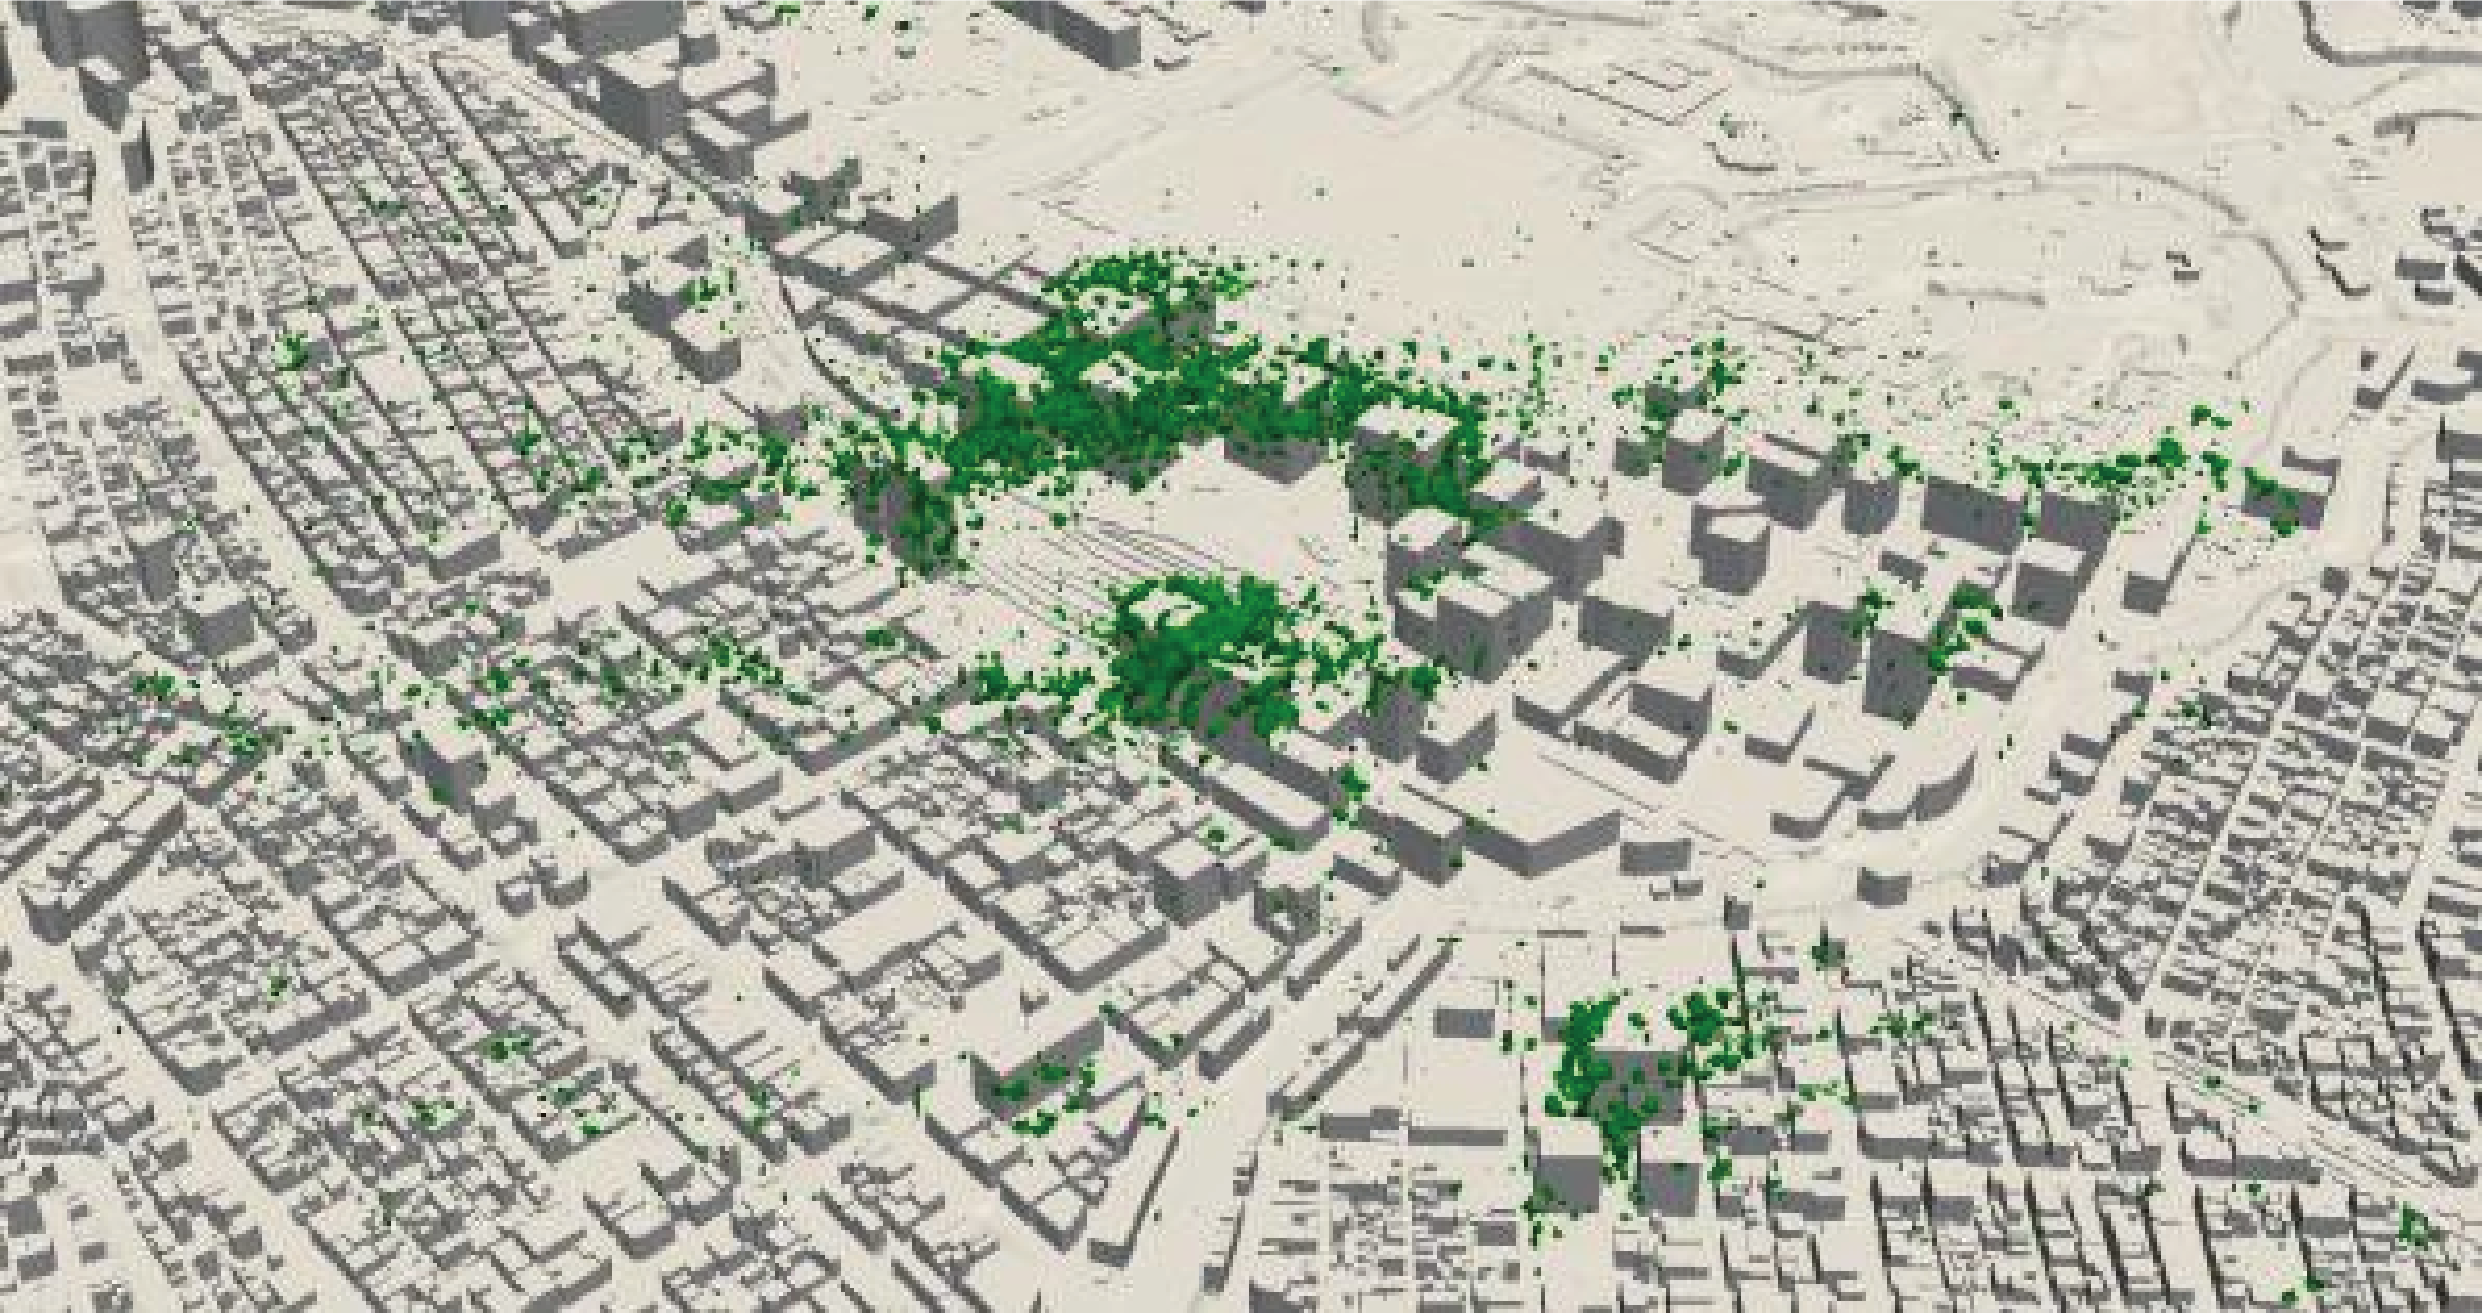
\includegraphics[height=3cm]
  {research/tsubokura/fig5_4.png}
  \caption{Q-criterion (Q=0.0015) in Marunouchi }
  \locallabel{fig54}
\end{figure}




\subsection{Development of unified compressible flow solver for unified low to moderate Mach number turbulence with hierarchical grid system}

The Simulation of the low speed compressible turbulence is a key challenge for the industrial applications such as combustion, aeroacoustics and significant heat transfer phenomena. Roe scheme with a low-Mach number fix [1] is adopted to tackle slow flows with variable densities. An immersed boundary method (IBM) for compressible flows with a fast, easy to implement and robust interpolation method is developed to handle the complex geometries.

{\bf Basic Validation with Academic case}: Based on the experiments conducted by Jia and Gogos [2], a steady-state natural convection around a heated sphere under the condition of that, the Grashof number based on the radius of the sphere is 104, is conducted to validate the unified solver. Fig. \localref{fig6a}(a) shows the contour of the velocity magnitude. The entrainment comes from the bottom of the sphere which is consistent with the description by [2]. Fig. \localref{fig6b} shows the temperature contour. Above the top of the sphere, higher temperature region is formed, which cause worse natural convection near the surface so the velocity in this region is quite low. Comparisons of the averaged Nusselt number (Nu), drag coefficients caused by pressure and viscous are tabulated in Table~\localref{tablecdcp}. The results are in good agreement with the experimental data and show the accuracy and availability of our program for dealing with the complex geometry and heat transfer problems. The present results have been published in [3].

\begin{figure}[h!]
\centering
  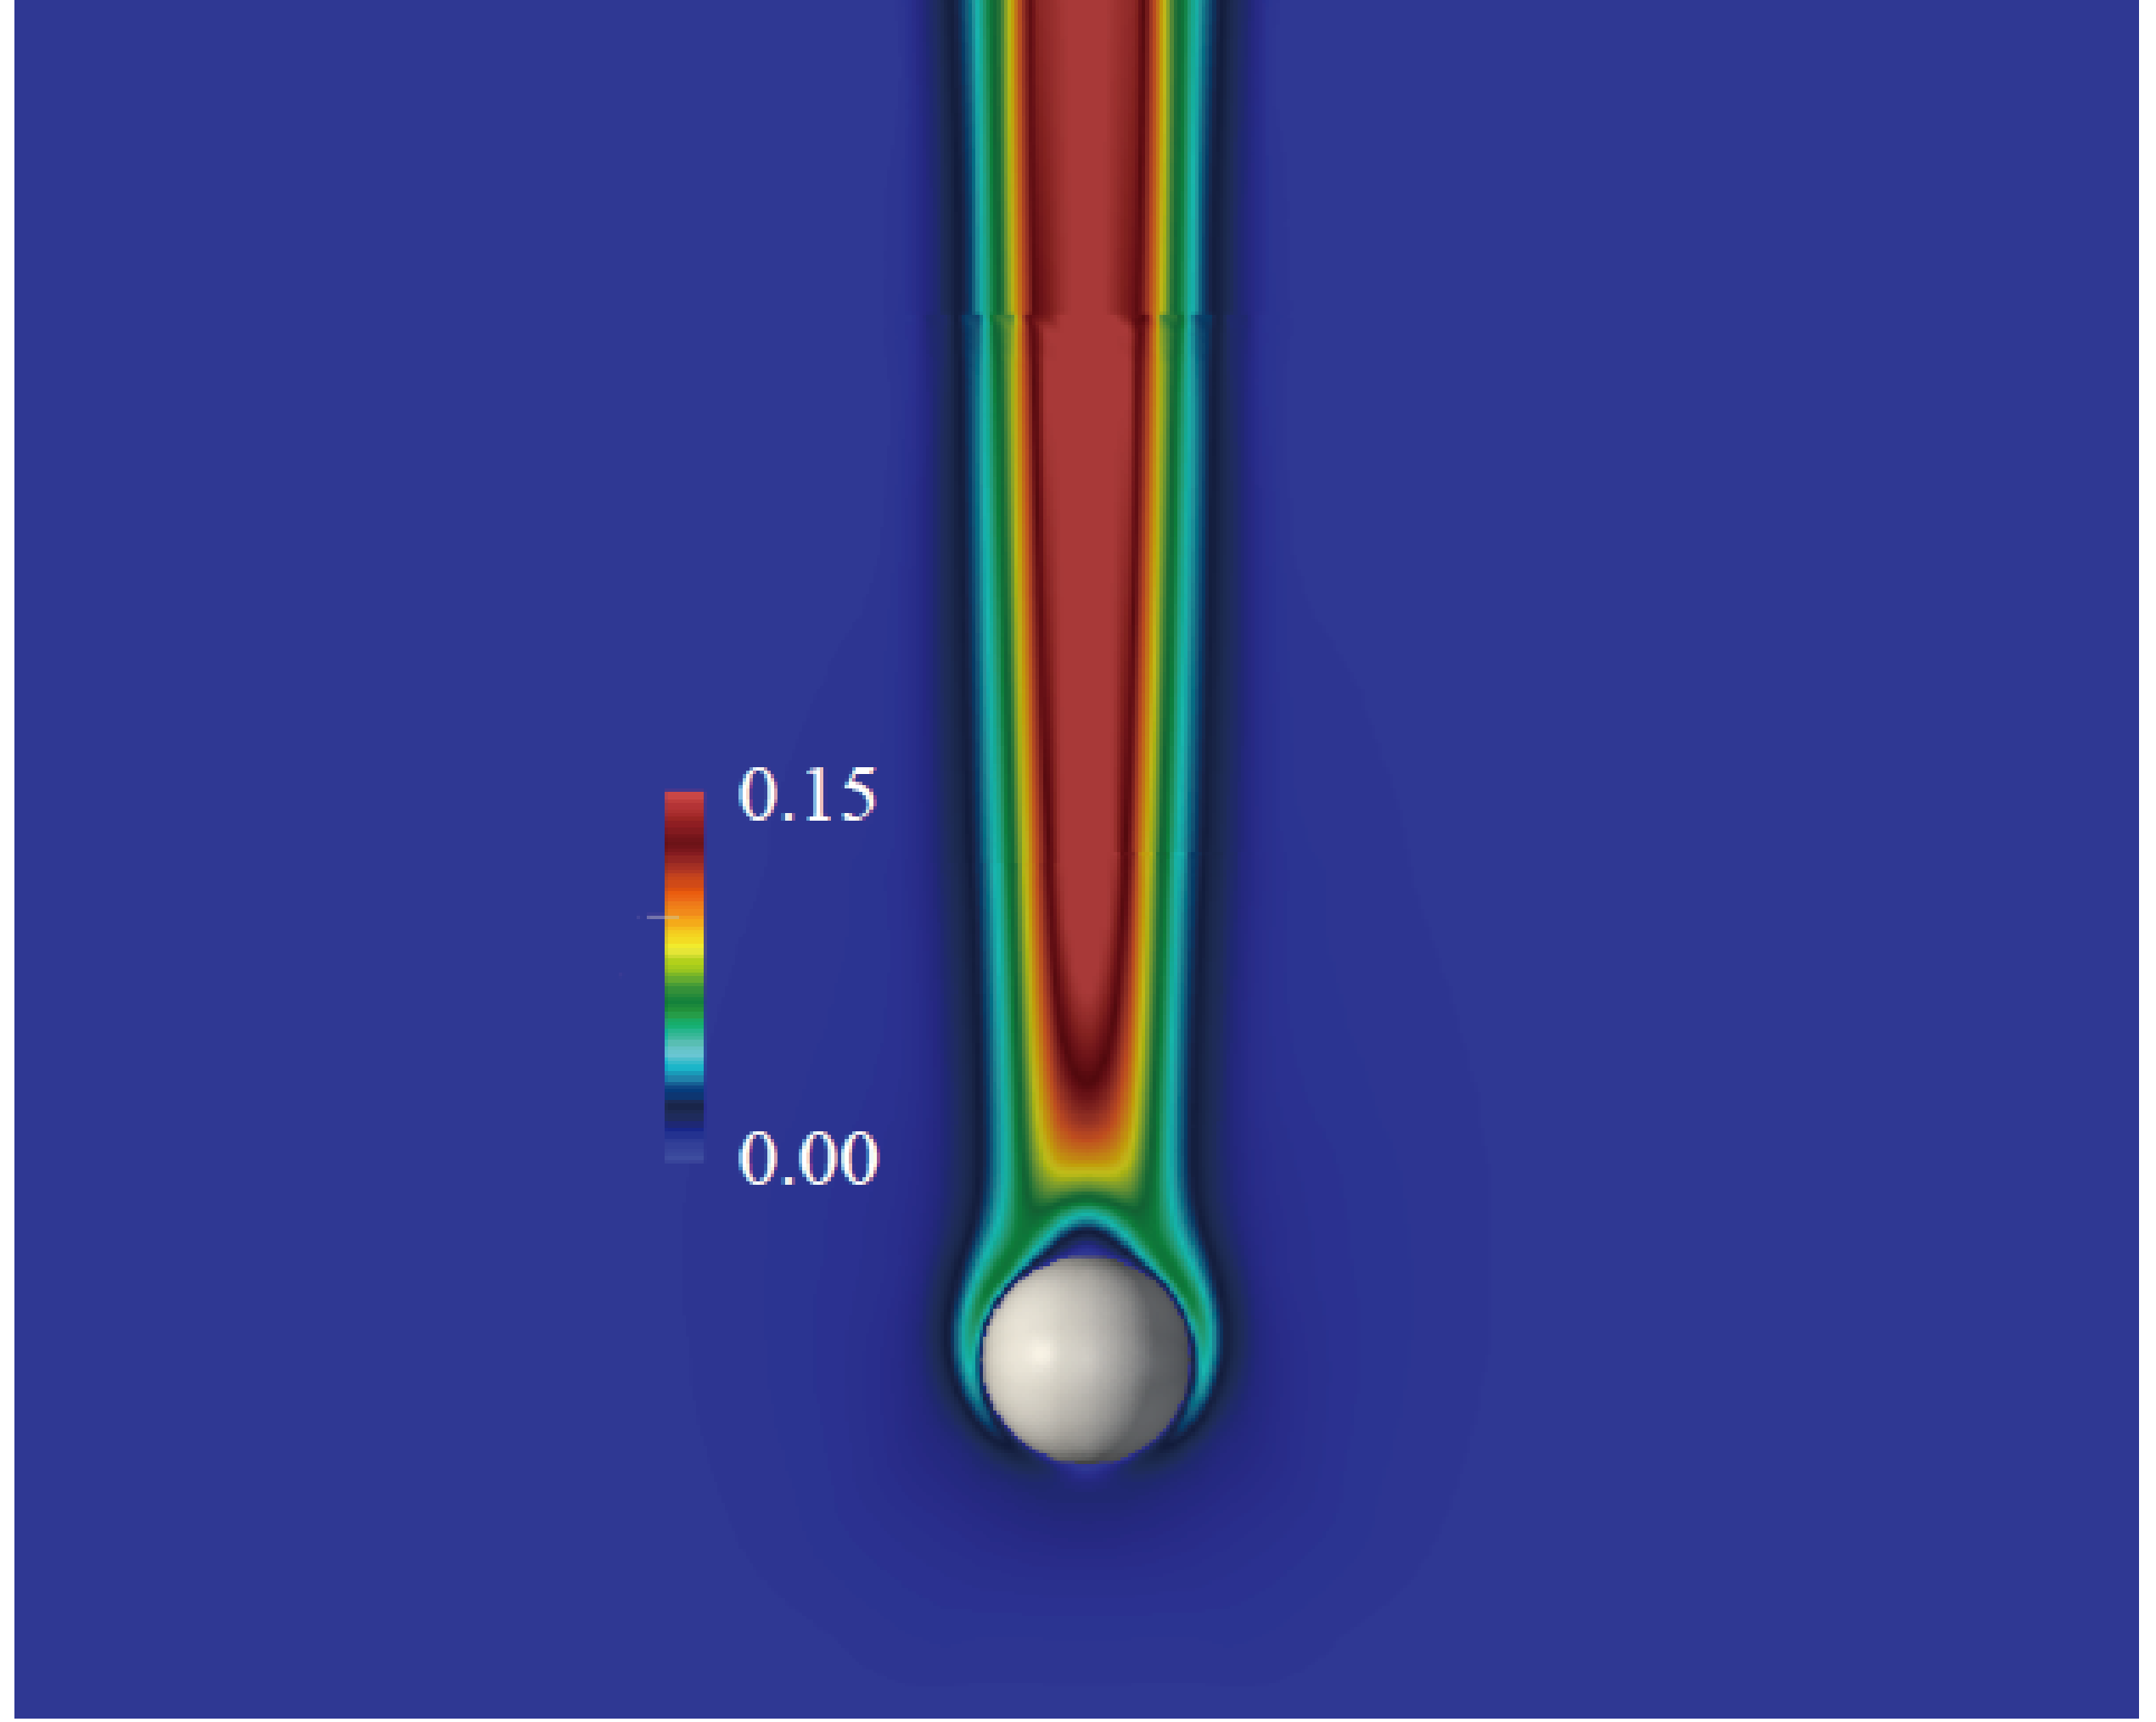
\includegraphics[height=5cm]
  {research/tsubokura/fig6a.png}
  \caption{A heated sphere: velocity magnitude (m/s) }
  \locallabel{fig6a}
\end{figure}

\begin{figure}[h!]
\centering
  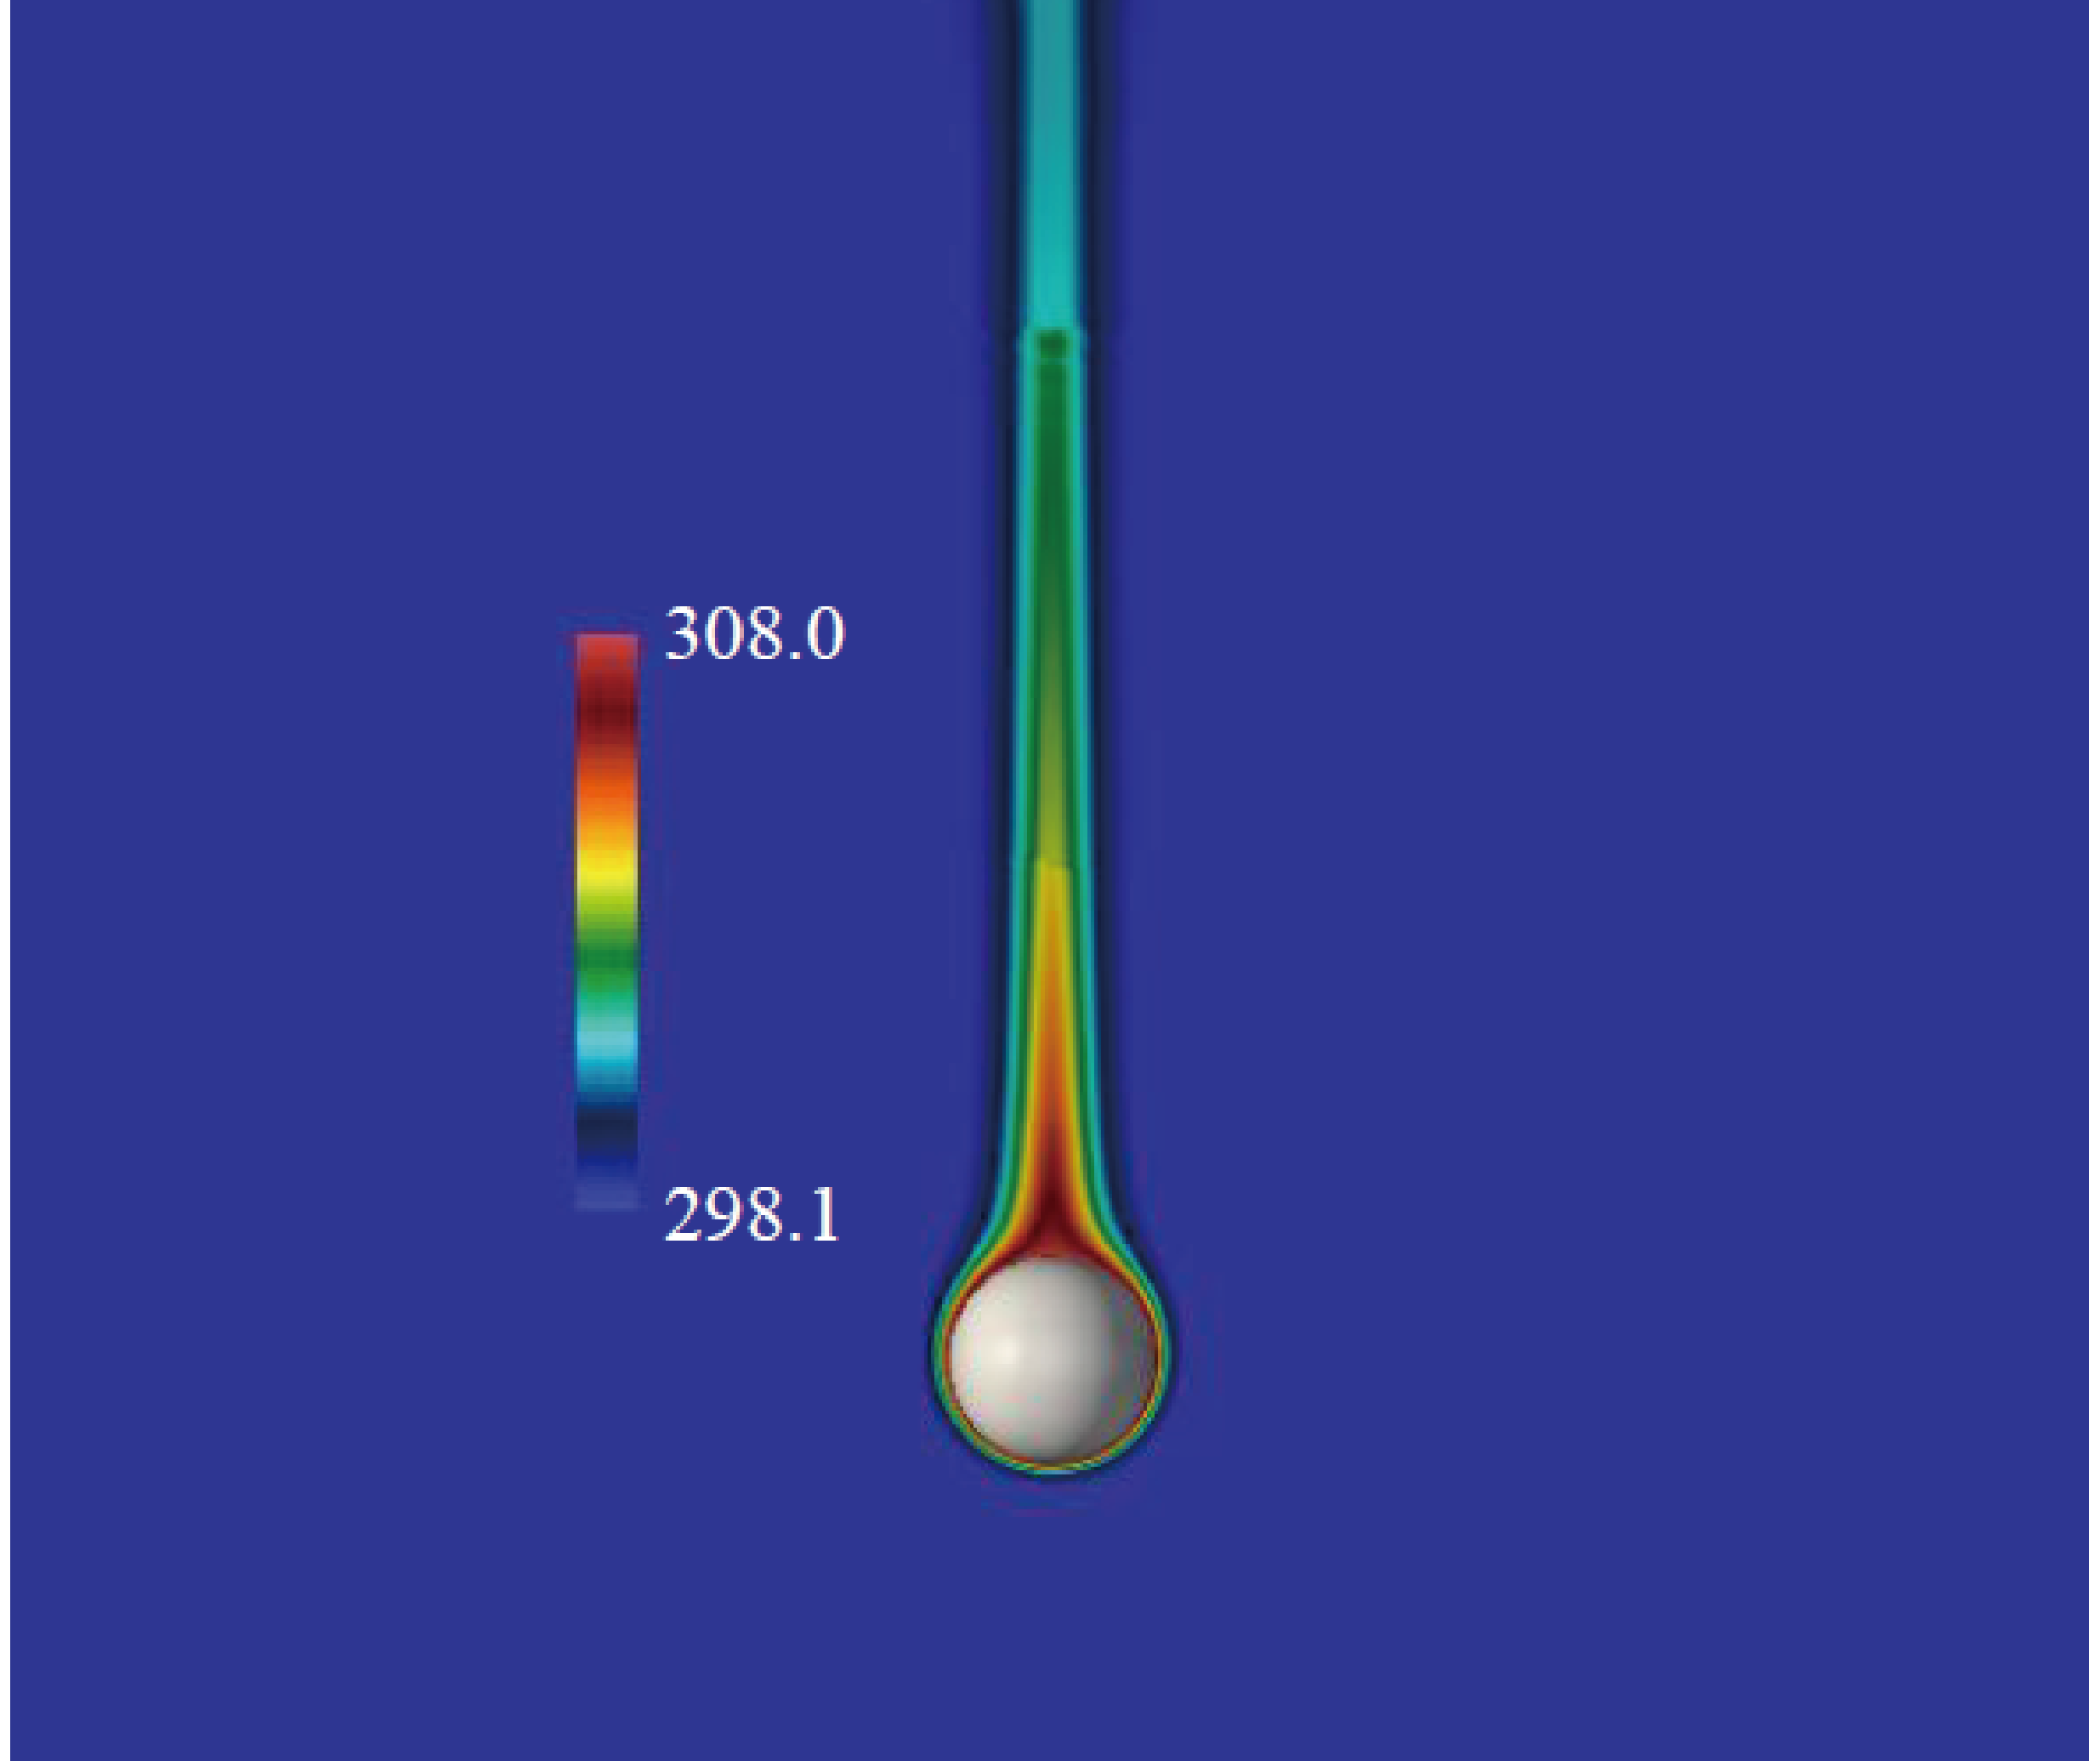
\includegraphics[height=5cm]
  {research/tsubokura/fig6b.png}
  \caption{A heated sphere:  temperature (K)}
  \locallabel{fig6b}
\end{figure}


\begin{table}[hbtp]
  \caption{Comparison with existing experimental data}
  \locallabel{tablecdcp}
  \centering
  \begin{tabular}{cccc}
    \hline
 & $\bar{Nu}$ & $C_{D,p}$ & $C_{D,u}$ \\
    \hline
Exp. [2] 	& 8.74	& 0.46	& 0.62 \\
Present	& 8.77	& 0.46	& 0.59 \\
    \hline
  \end{tabular}
\end{table}


The simulation of a sphere at Re=104 is performed to investigate the availability of the unified solver for higher Reynolds numbers. Fig. \localref{figmpc} shows the distribution of mean pressure coefficient. The result is well consistent with the [4] and the separation angle can be also accurately captured, which is around 86 degrees.

Fig. \localref{figshcrite} shows the Q criterion contoured by the magnitude of the velocity. The turbulence structures are mainly formed after the separated shear layers generated from the separation point. Besides, the transition from large to small turbulence structures can be also clearly observed in the wake region.

\begin{figure}[h!]
\centering
  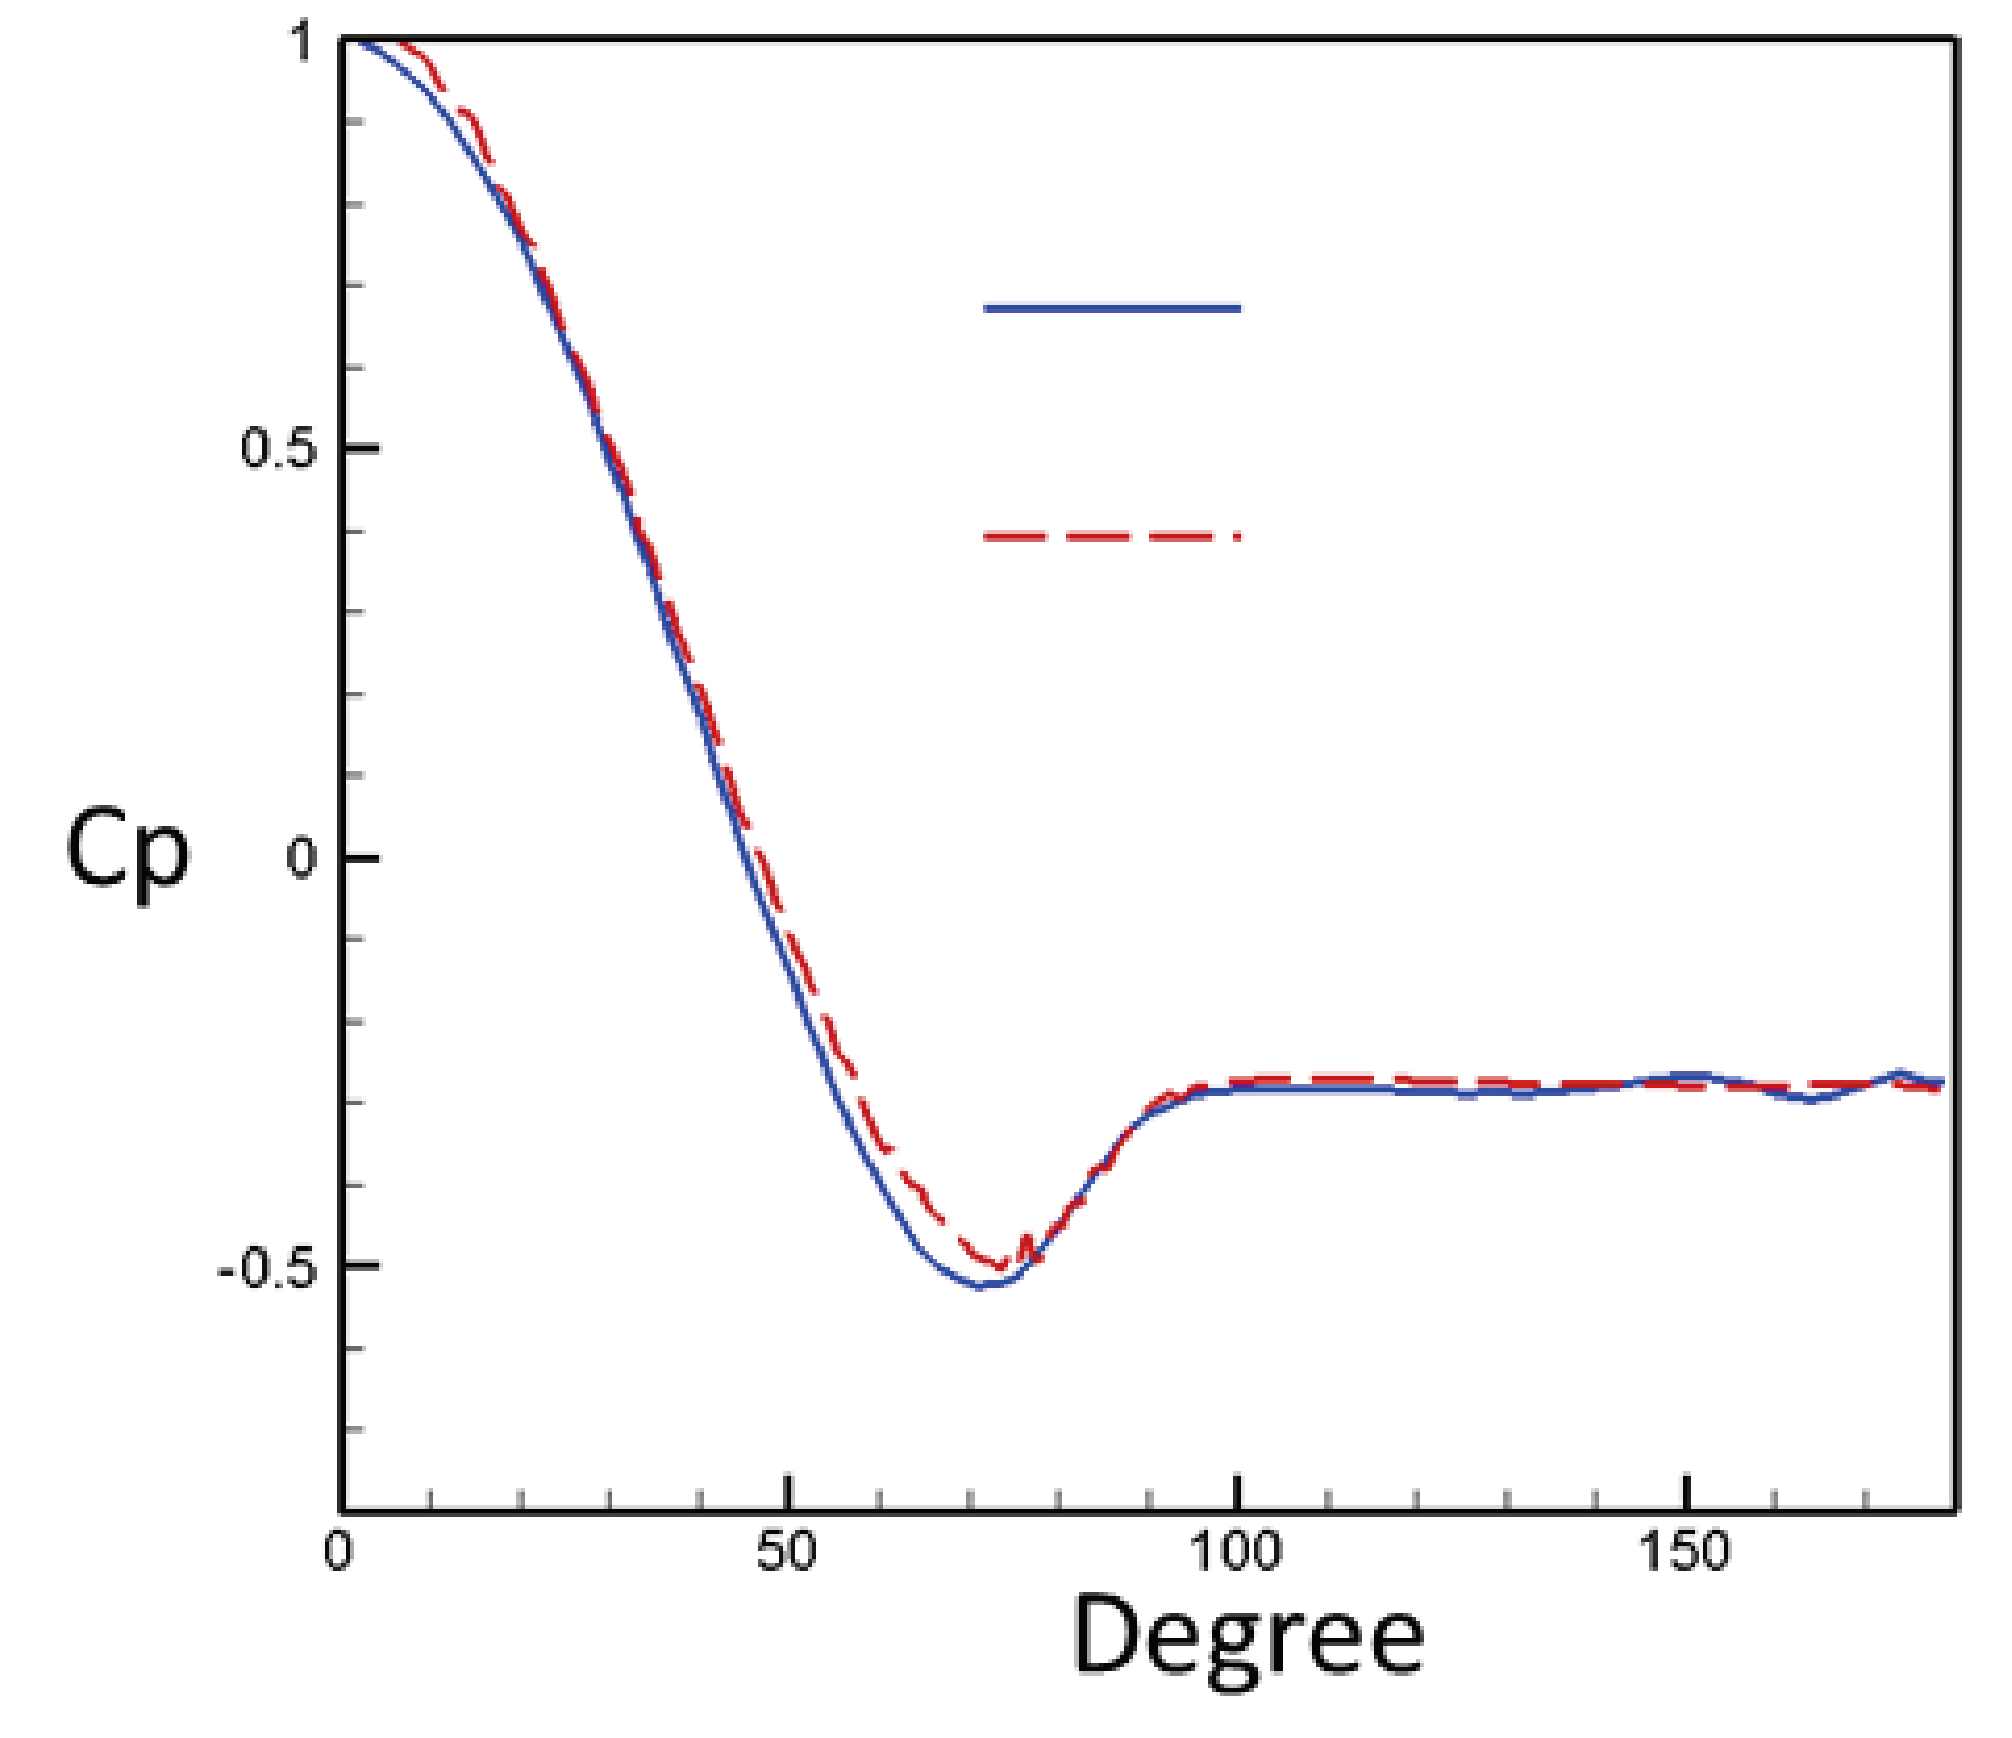
\includegraphics[height=5cm]
  {research/tsubokura/fig7a.png}
  \caption{Sphere flow at Re=$10^4$: Distribution of mean pressure coefficient}
  \locallabel{figmpc}
\end{figure}

\begin{figure}[h!]
\centering
  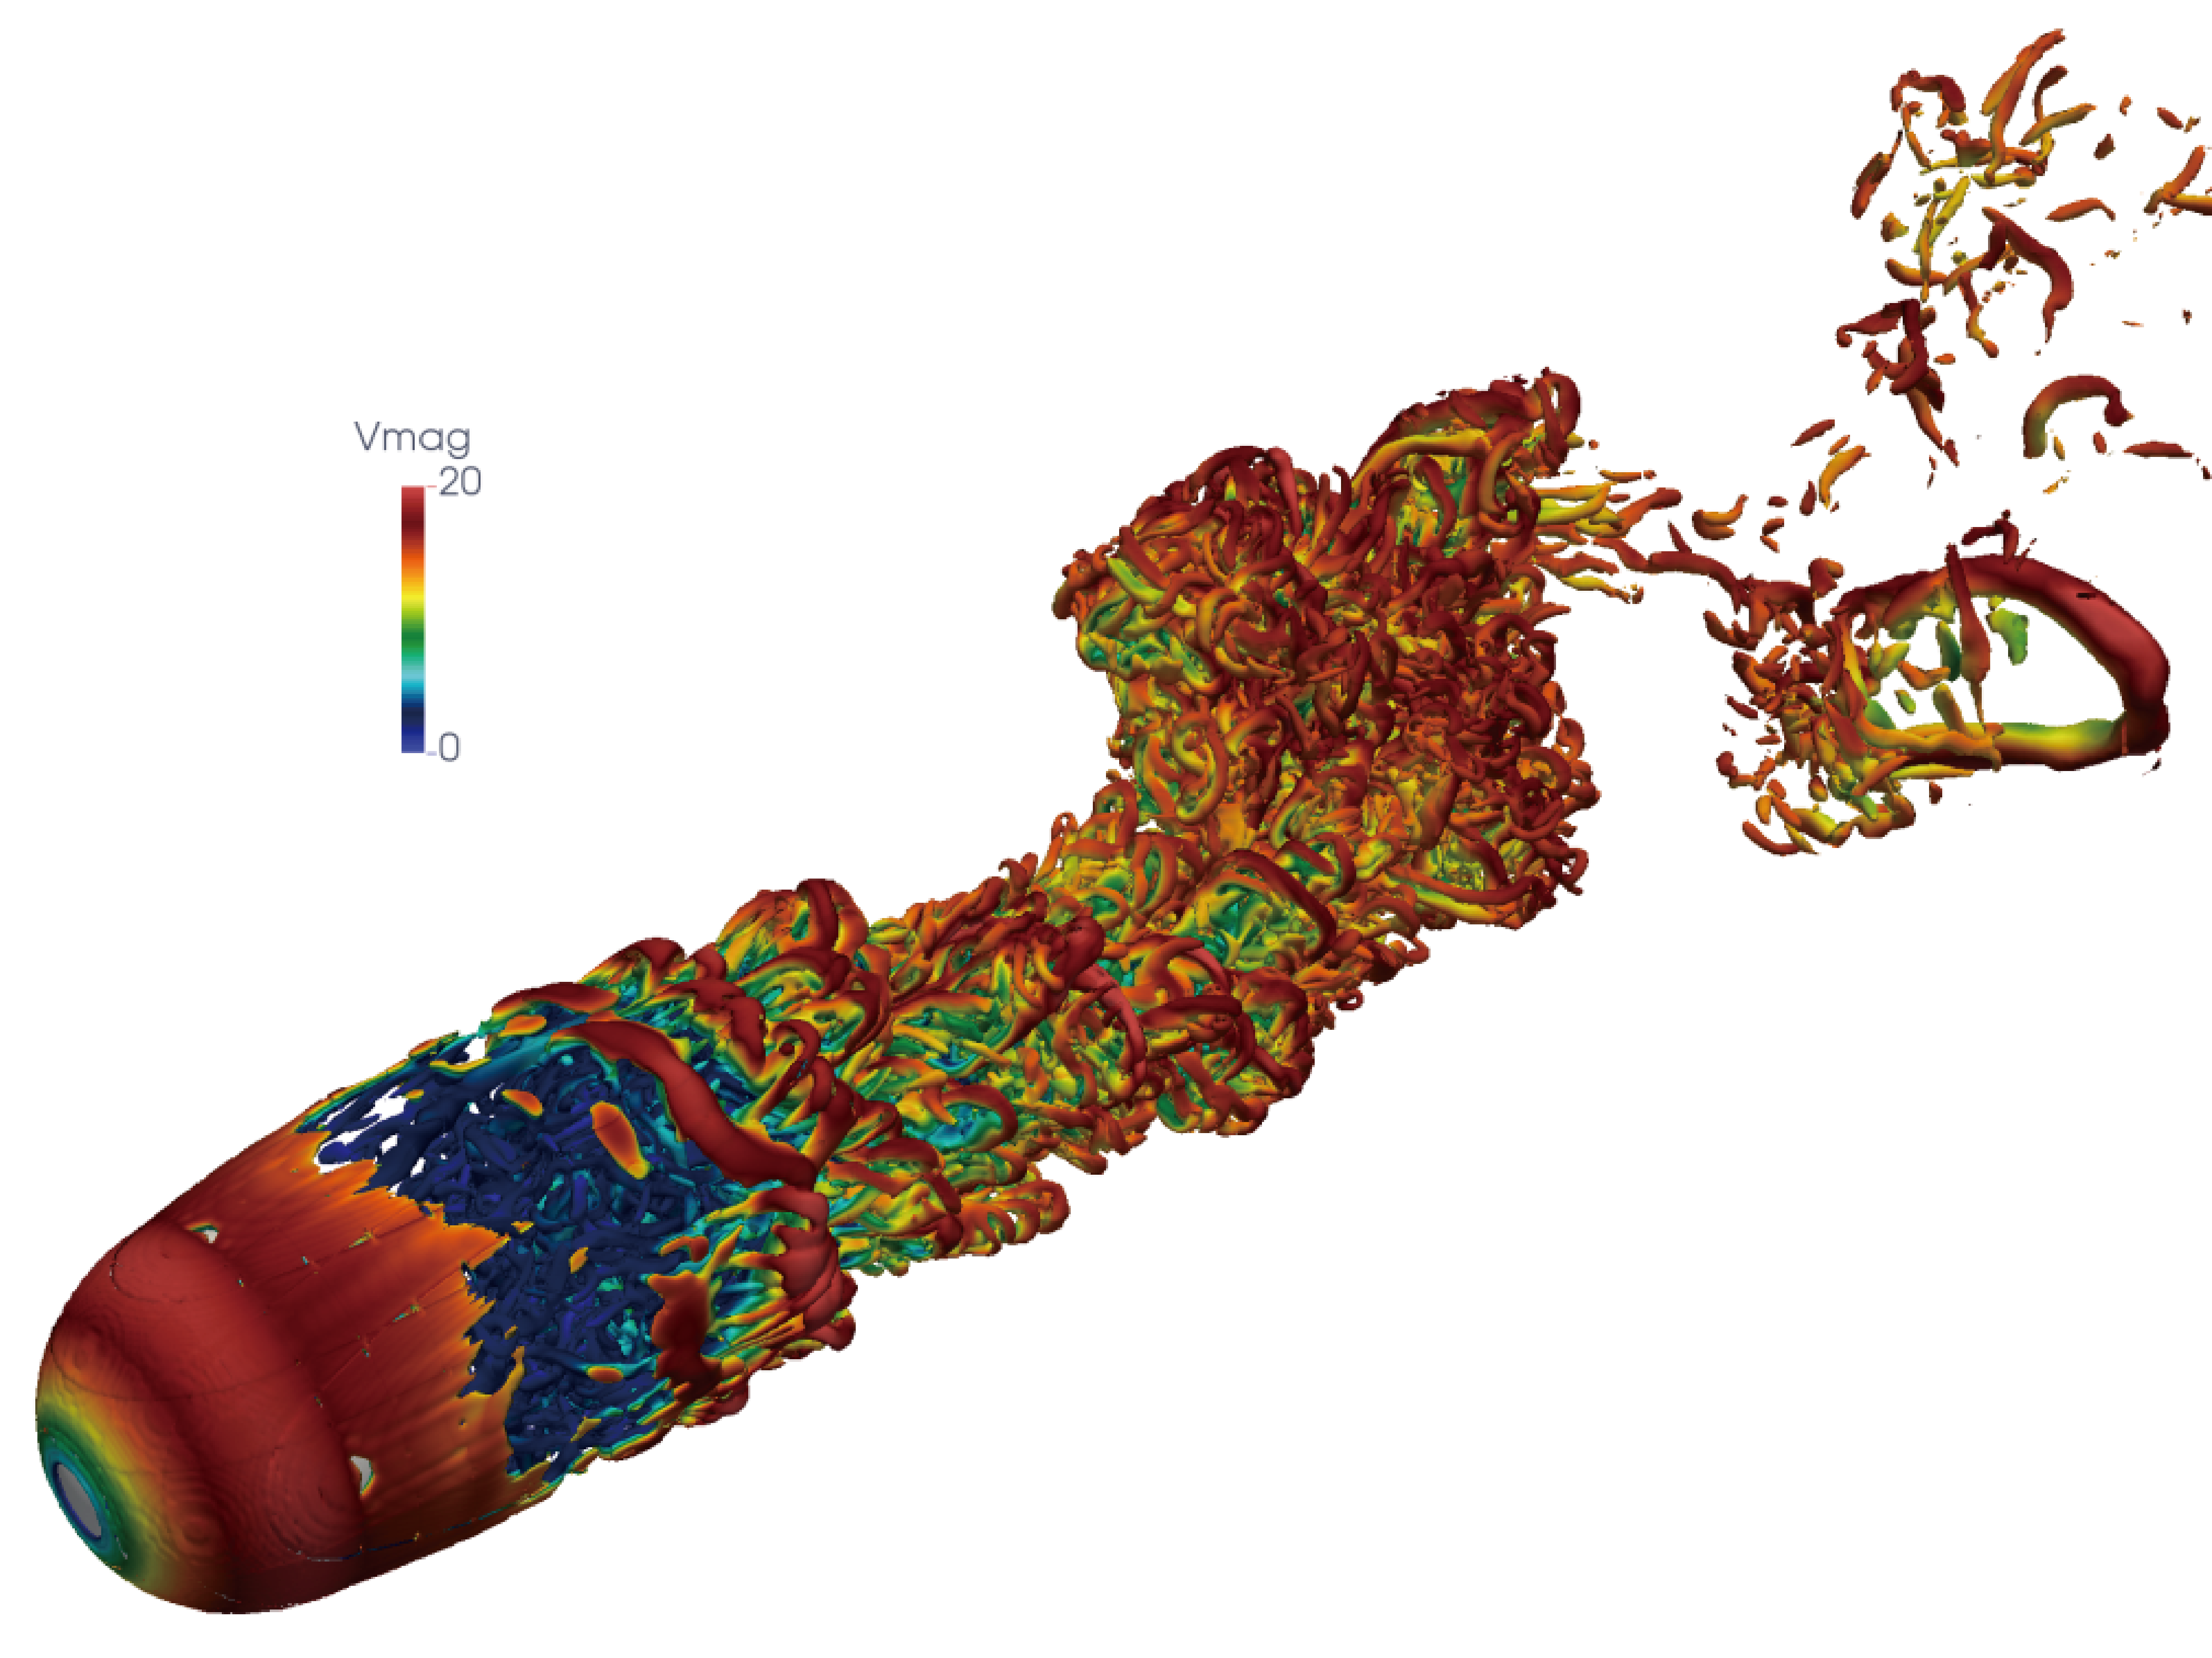
\includegraphics[height=5cm]
  {research/tsubokura/fig7b.png}
  \caption{Sphere flow at Re=$10^4$: Q criterion}
  \locallabel{figshcrite}
\end{figure}


Finally, the simulation of the whole vehicle demonstrates the capability of the unified solver. Fig. \localref{figvelsimvelmag} shows the contour of the velocity magnitude. The development of the boundary layer on the front window and roof can be clearly observed, which shows the capability of unified solver for handling the complex geometry. Besides, the flows penetrate the front of the car to the engine room is also obviously shown, which indicates that our immersed boundary can also treat non-watertight geometry. Fig. \localref{figvstimes} shows the history of the drag and lift coefficients. After reaching the quasi steady state, the average vales of them are good agreement with the experimental data. This is an indication that the unified solver is also able to obtain accurate results for this kind of practical application. In Fig. \localref{figvsflowstr}, the Q-criterion contoured by the magnitude of velocity is shown. The development of turbulent coherent structures near the wheel, mirror and side windows is well captured. In addition, the typical turbulent structures-hair pin can be also obviously observed on the roof.

\begin{flushleft}
[1] F. Rieper, Journal of Computational Physics, 230 (2011) 5263-5287.

[2] H. Jia, G. Gogos, Int. J. Heat Mass Transfer 19 (1996) 1603-1615.

[3] C. Li, M. Tsubokura, Int. J. Heat Mass Transfer 75 (2016) 52-58.

[4] C. George, S. Kyle, Physics of Fluids, 16 (2004) 1449-1466.
\end{flushleft}

\begin{figure}[h!]
\centering
  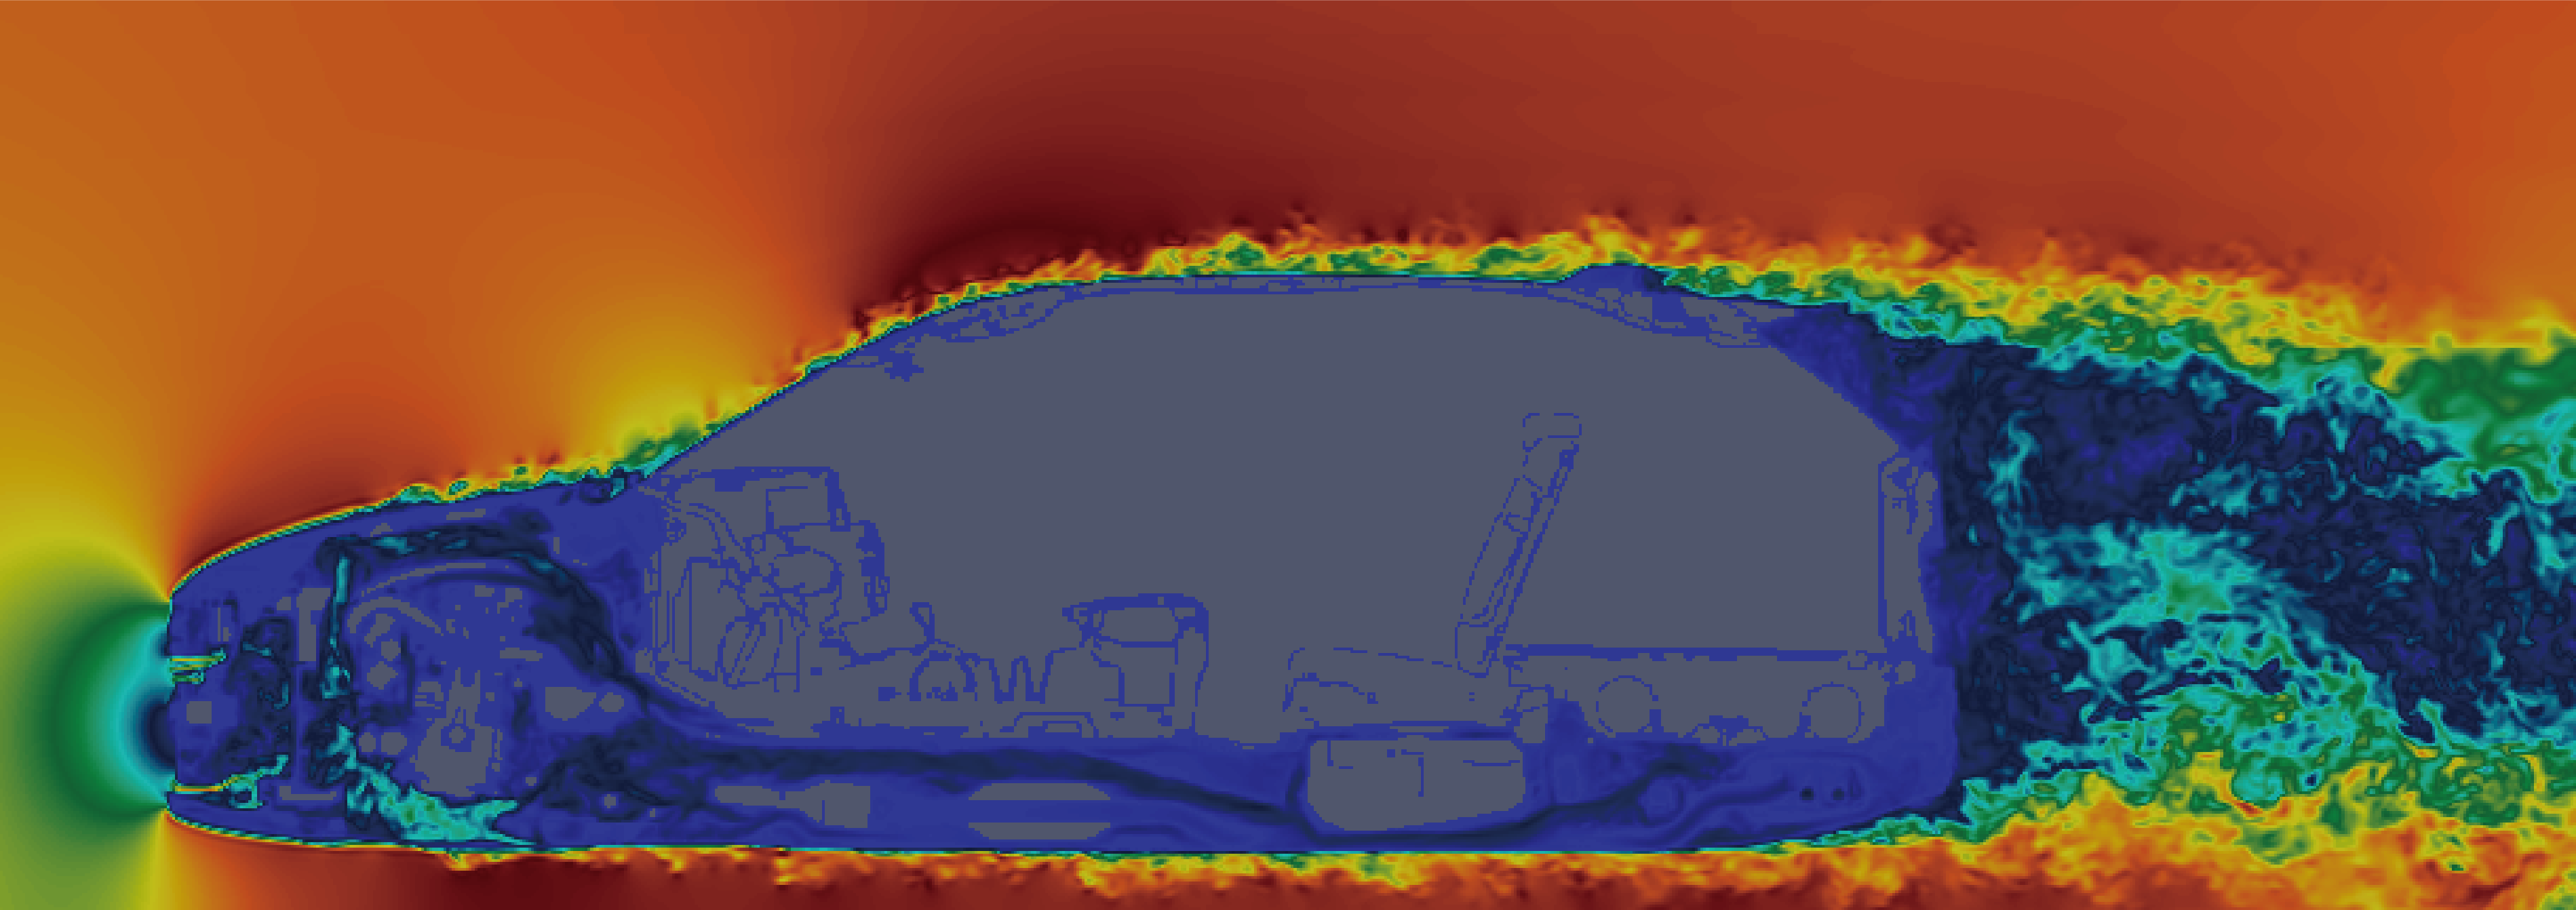
\includegraphics[height=3cm]
  {research/tsubokura/fig8a.png}
  \caption{Vehicle Simulation: Snapshot of velocity magnitude}
  \locallabel{figvelsimvelmag}
\end{figure}

\begin{figure}[h!]
\centering
  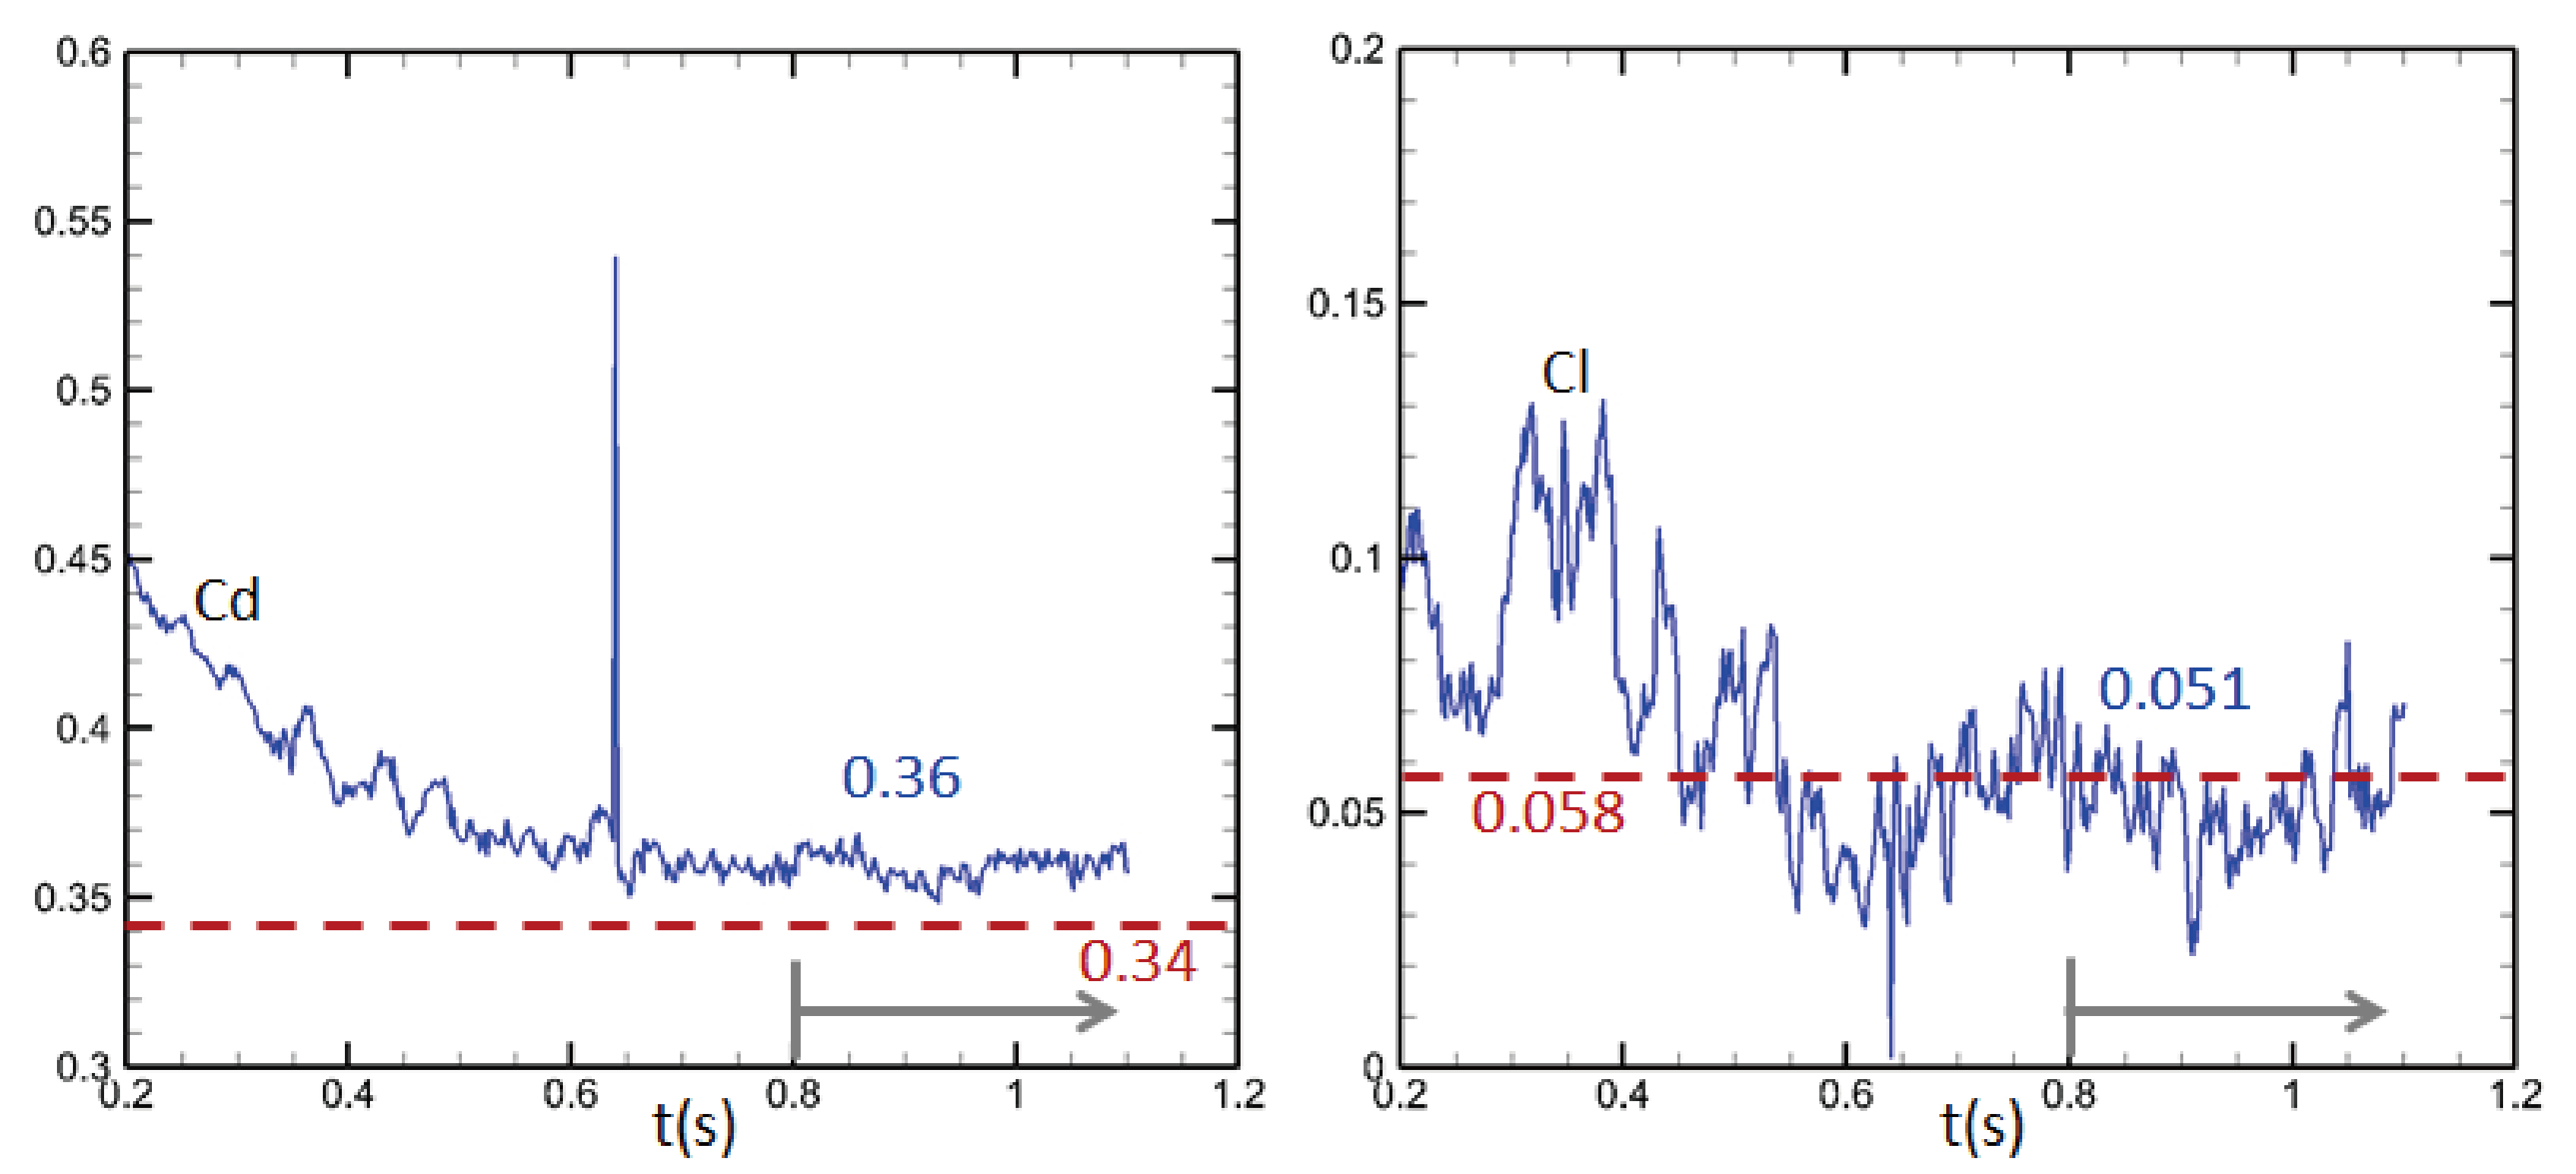
\includegraphics[height=5cm]
  {research/tsubokura/fig8b.png}
  \caption{Vehicle Simulation: Time series of drag (left) and lift (right) coefficients}
  \locallabel{figvstimes}
\end{figure}

\begin{figure}[h!]
\centering
  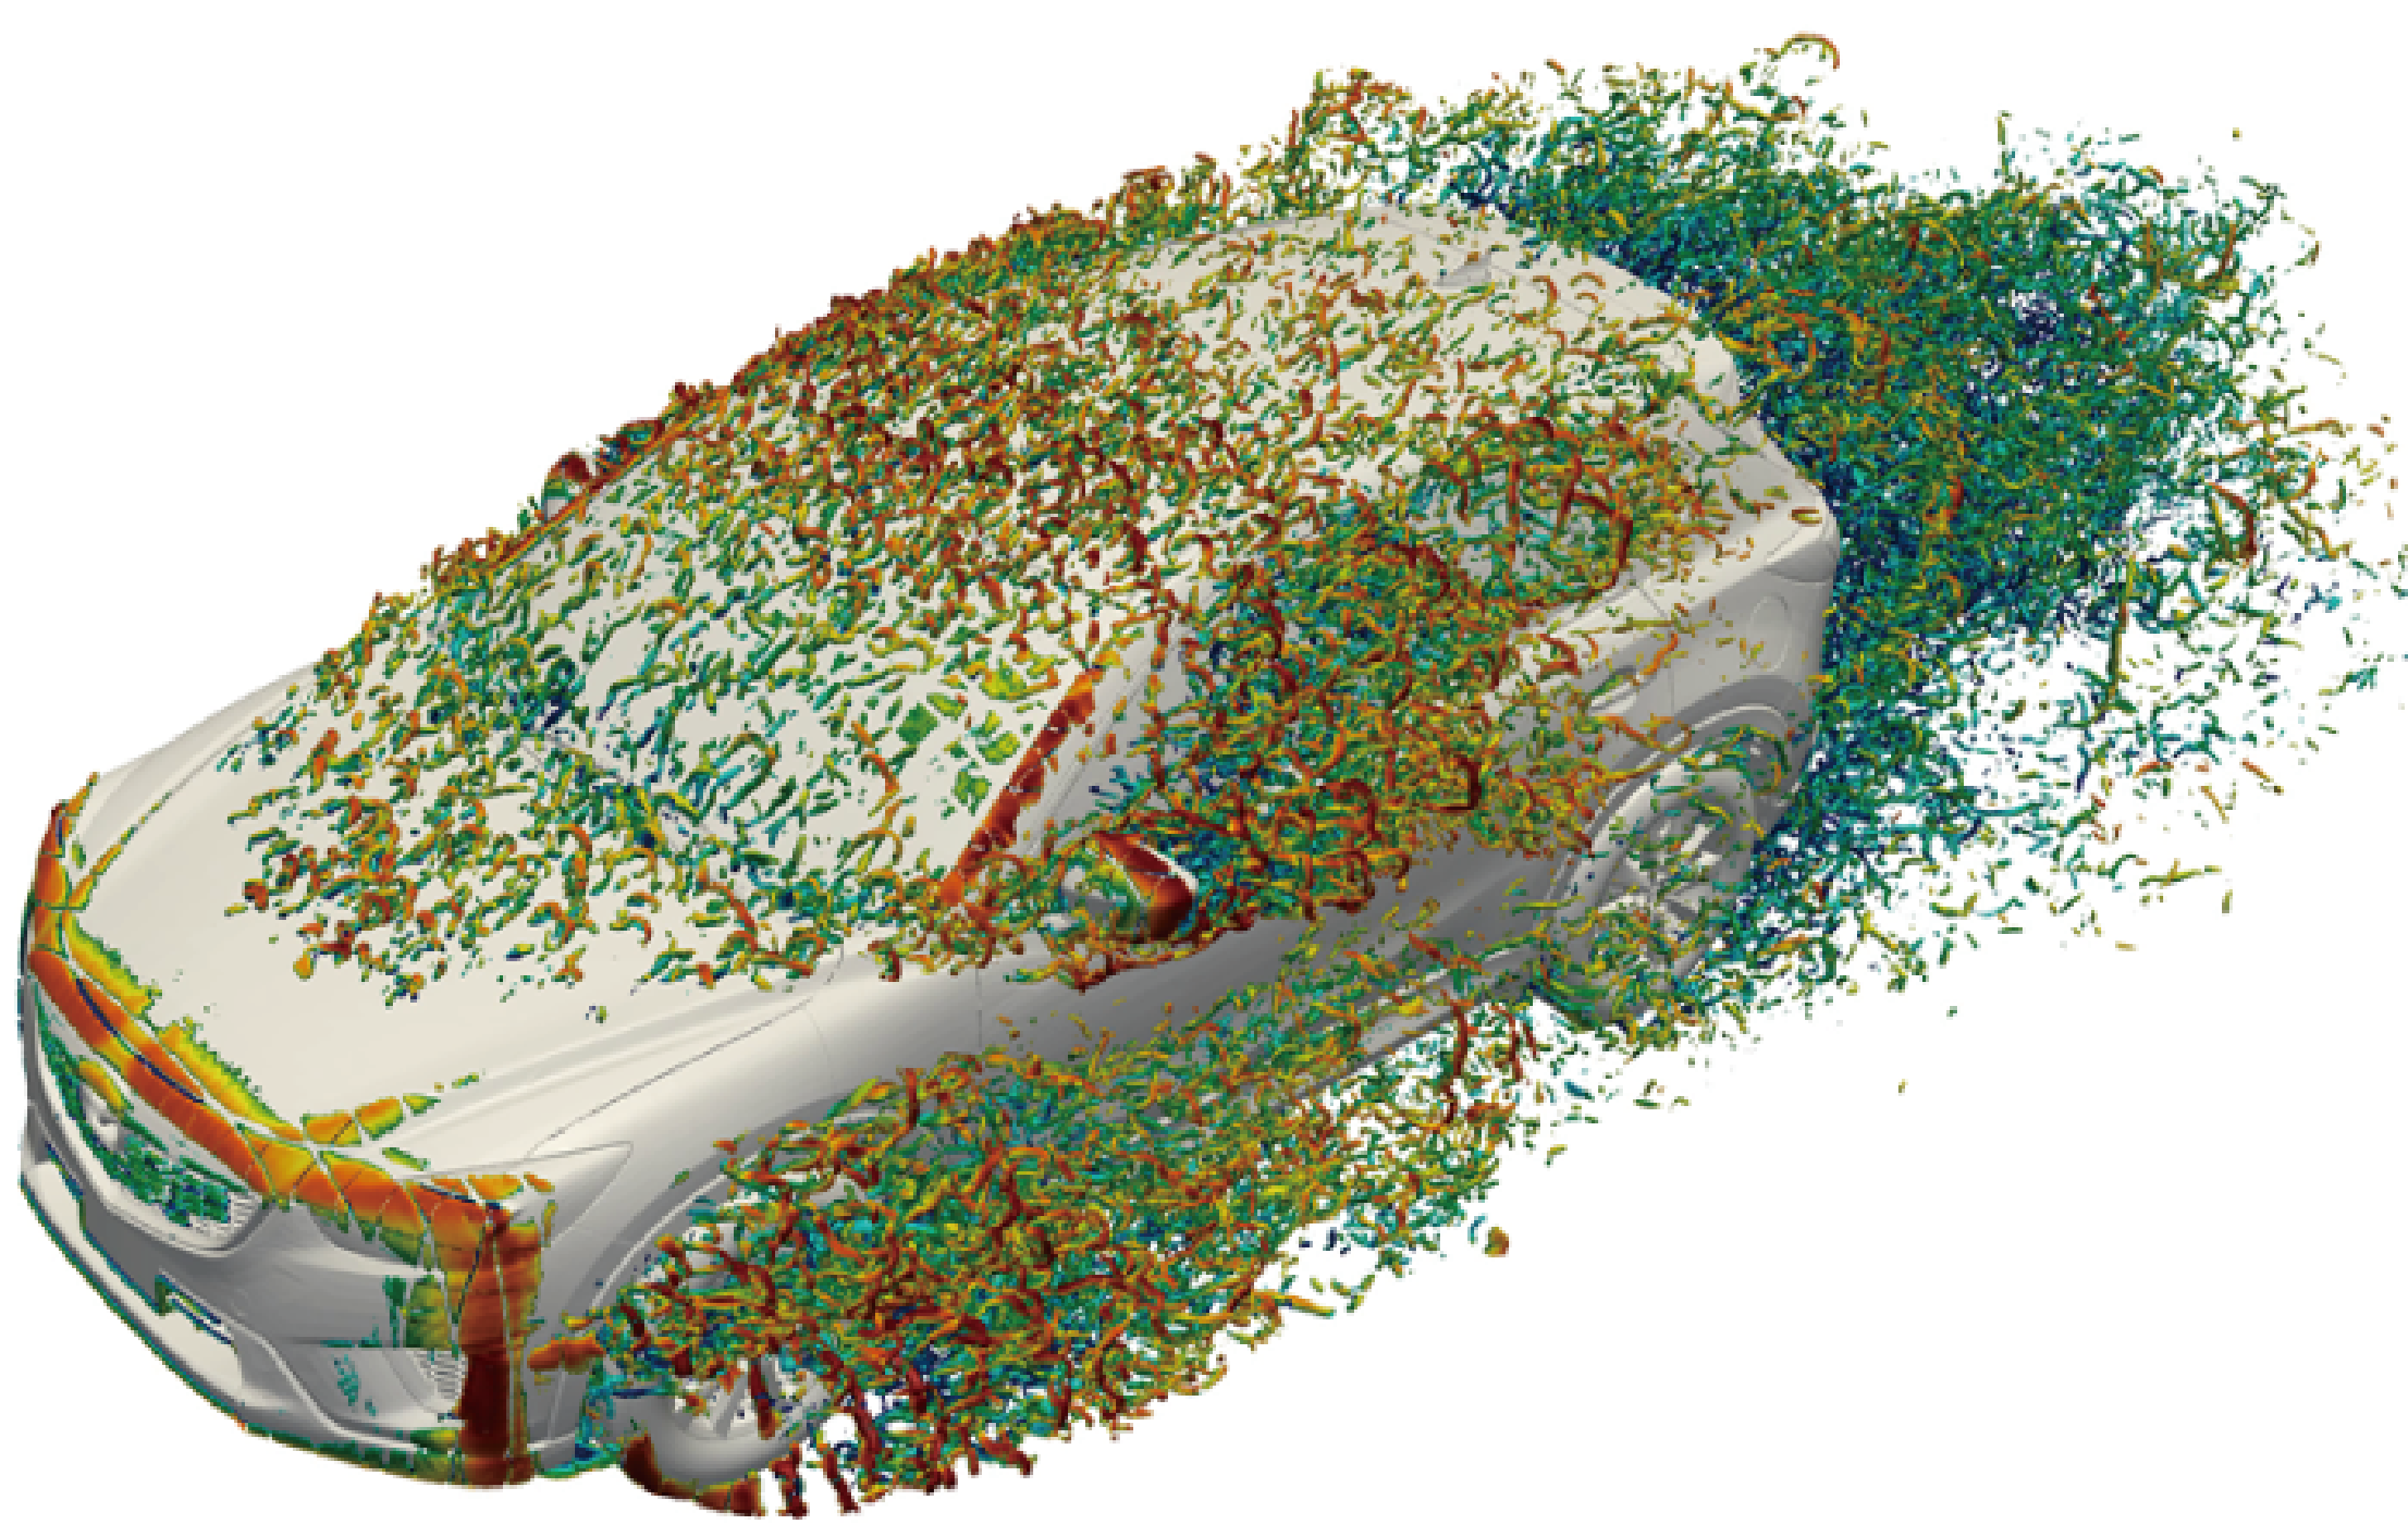
\includegraphics[height=6cm]
  {research/tsubokura/fig8c.png}
  \caption{Vehicle Simulation: Snapshot of flow structures extracted by the Q-criterion}
  \locallabel{figvsflowstr}
\end{figure}


\subsection{Development of high performance moving boundary solver for realistic motion}
{\bf Aerodynamics of Vehicle in a turn}: The aerodynamic performance and stability a vehicle is strongly influenced by the crosswinds during cruise and while in turning maneuvers. It is difficult to simulate such real-world flow scenarios in wind tunnel experiments. Furthermore, it is also difficult to measure unsteady aerodynamic forces in wind tunnel experiments. Thus, it is desirable for numerical methods to be able to efficiently and accurately simulate such flow conditions. To this end, here, we present simulation of a vehicle (the complex full vehicle geometry discussed in the previous section) undergoing a turning motion, including wheel rotation and turn, chassis roll and turn, in a uniform flow. This simulation the result of a collaborative work between Mazda Motor Corporation and RIKEN AICS. The detailed vehicle geometry and it motion data were provided by Mazda, and the simulation was carried out at on the K-computer using CUBE. The Lagrangian-Eulerian approach developed during the previous year was used for this simulation. As mentioned above all the vehicle motion, except linear translation, is imposed on the vehicle. If the linear translational motion was imposed on the vehicle, a fine mesh would be needed in the vehicle's path, which makes the mesh size excessively large. An alternate approach, where instead of imposing the linear translation on the vehicle it is imposed on the entire mesh, was used. In this approach the vehicle's center of gravity remains fixed relative to the mesh. So, the fine mesh is needed only in a small region around the vehicle instead of the region of the vehicle's path. This reduced the mesh size by a factor of 3-5.   The results of the simulations are shown in Fig. \localref{figffavitrn}.

\begin{figure}[h!]
\centering
  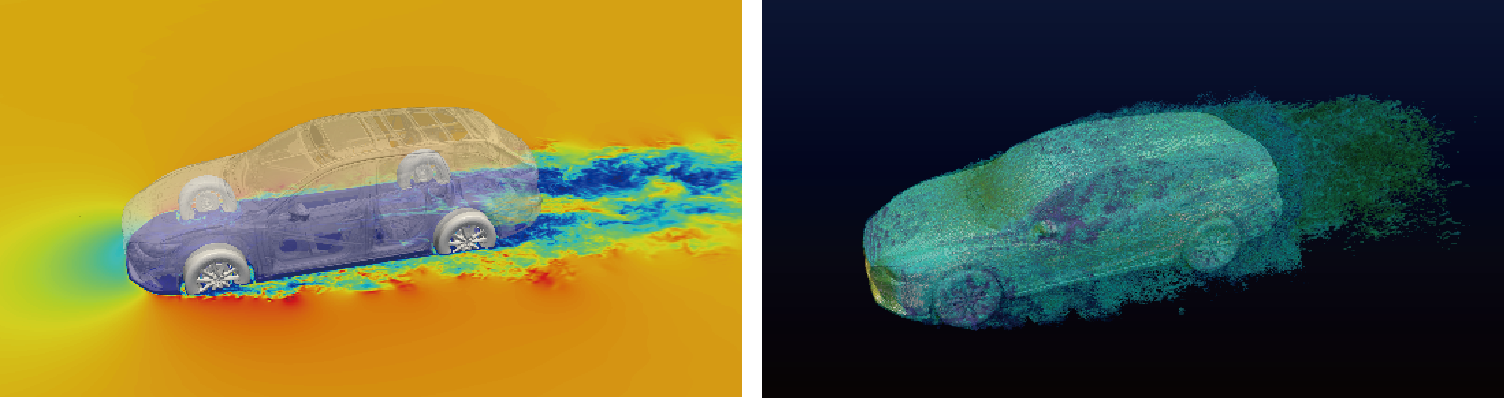
\includegraphics[height=4cm]
  {research/tsubokura/fig9.png}
  \caption{Flow field around a vehicle in a turn. (Left) Velocity magnitude on a horizontal plane. (Right) Iso surface of swirl. }
  \locallabel{figffavitrn}
\end{figure}


{\bf Aerodynamic performance of a Ski jumper}: Ski jump is a popular winter sport and is a part of winter Olympics. It is one of the sports in which Japan is competitive and has some of the best ski jumpers in the world. Ski Jump is a sport where aerodynamic interaction of the jumper and air plays a key role in outcome of the sport. Minute changes in an athlete's posture can go a long way, literally.  The distance covered by an athlete is strongly correlated to the drag and lift forces on the athlete while in air. And, these forces are greatly influenced by the athlete's posture. In collaboration with Prof. Keizo Yamamoto of Hokusyo University we investigated the aerodynamic performance of two of Japan's top ski jump athletes, Haruka Iwasa and Sara Takanashi.  Through the unsteady aerodynamic simulation of the two ski jumpers we analyzed the evolution of forces during a short period before and after the jump from the ski ramp. During this period the jumper changes from a sitting posture to a standing posture. Our analysis revealed that the posture and motion of Haruka Iwasa lead to lower drag force and higher lift force compared to the forces on Sara Takanashi. This is consistent with the real-world performance record of the two ski-jumpers.

\begin{figure}[h!]
\centering
  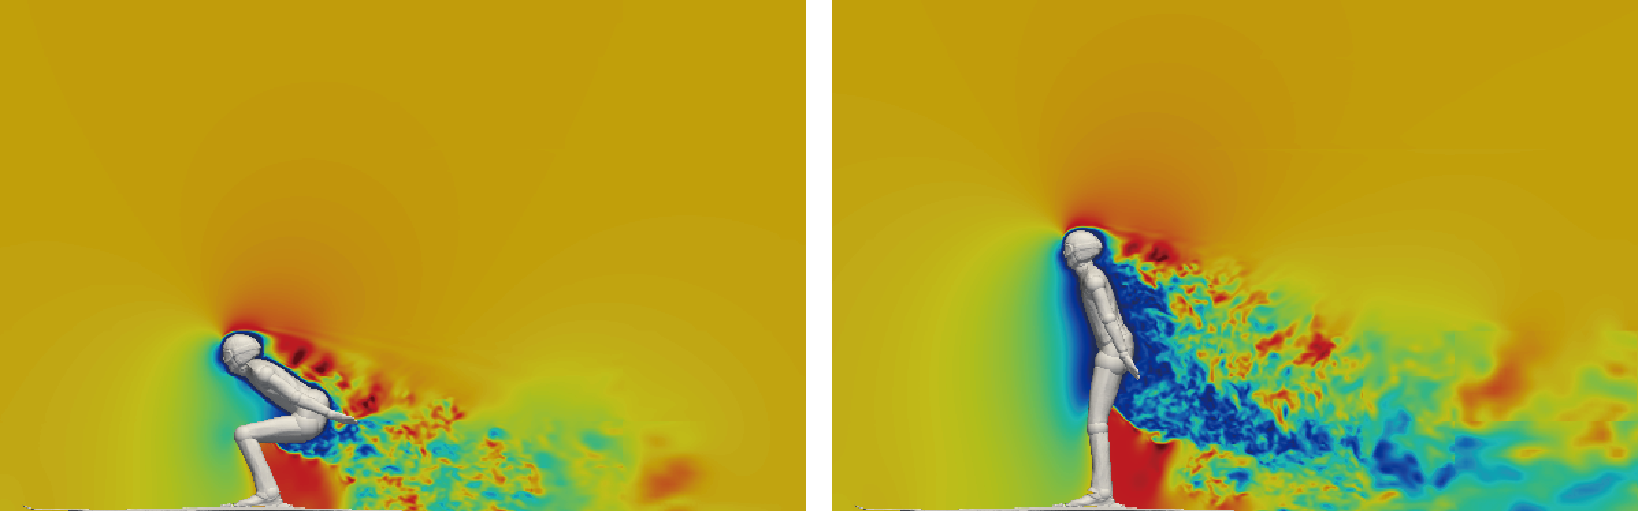
\includegraphics[height=4.5cm]
  {research/tsubokura/fig10.png}
  \caption{Evolution of flow around Ski jumper Haruka Iwasa during a jump. (Left) Starting posture of the jump. (Right) Final posture of the jump.}
  \locallabel{fig10}
\end{figure}

\section{Schedule and Future Plan}

\subsection*{(1)Five-year objectives and goals toward 2017}
\begin{itemize}
 \item Construction and development of the simulation technology for bringing out the performance of K-computer
 \item Proposal of the technological trend of HPC simulation toward EXA-scale
\end{itemize}


\subsection*{(2)Long-term objectives}
\begin{itemize}
 \item Establishment of the research and development center for industrial simulation technology
 \item Contribution to computer science by expanding the developed simulation technology to different fields
\end{itemize}


\subsection*{(3)Time schedule}
\begin{figure}[h!]
\centering
  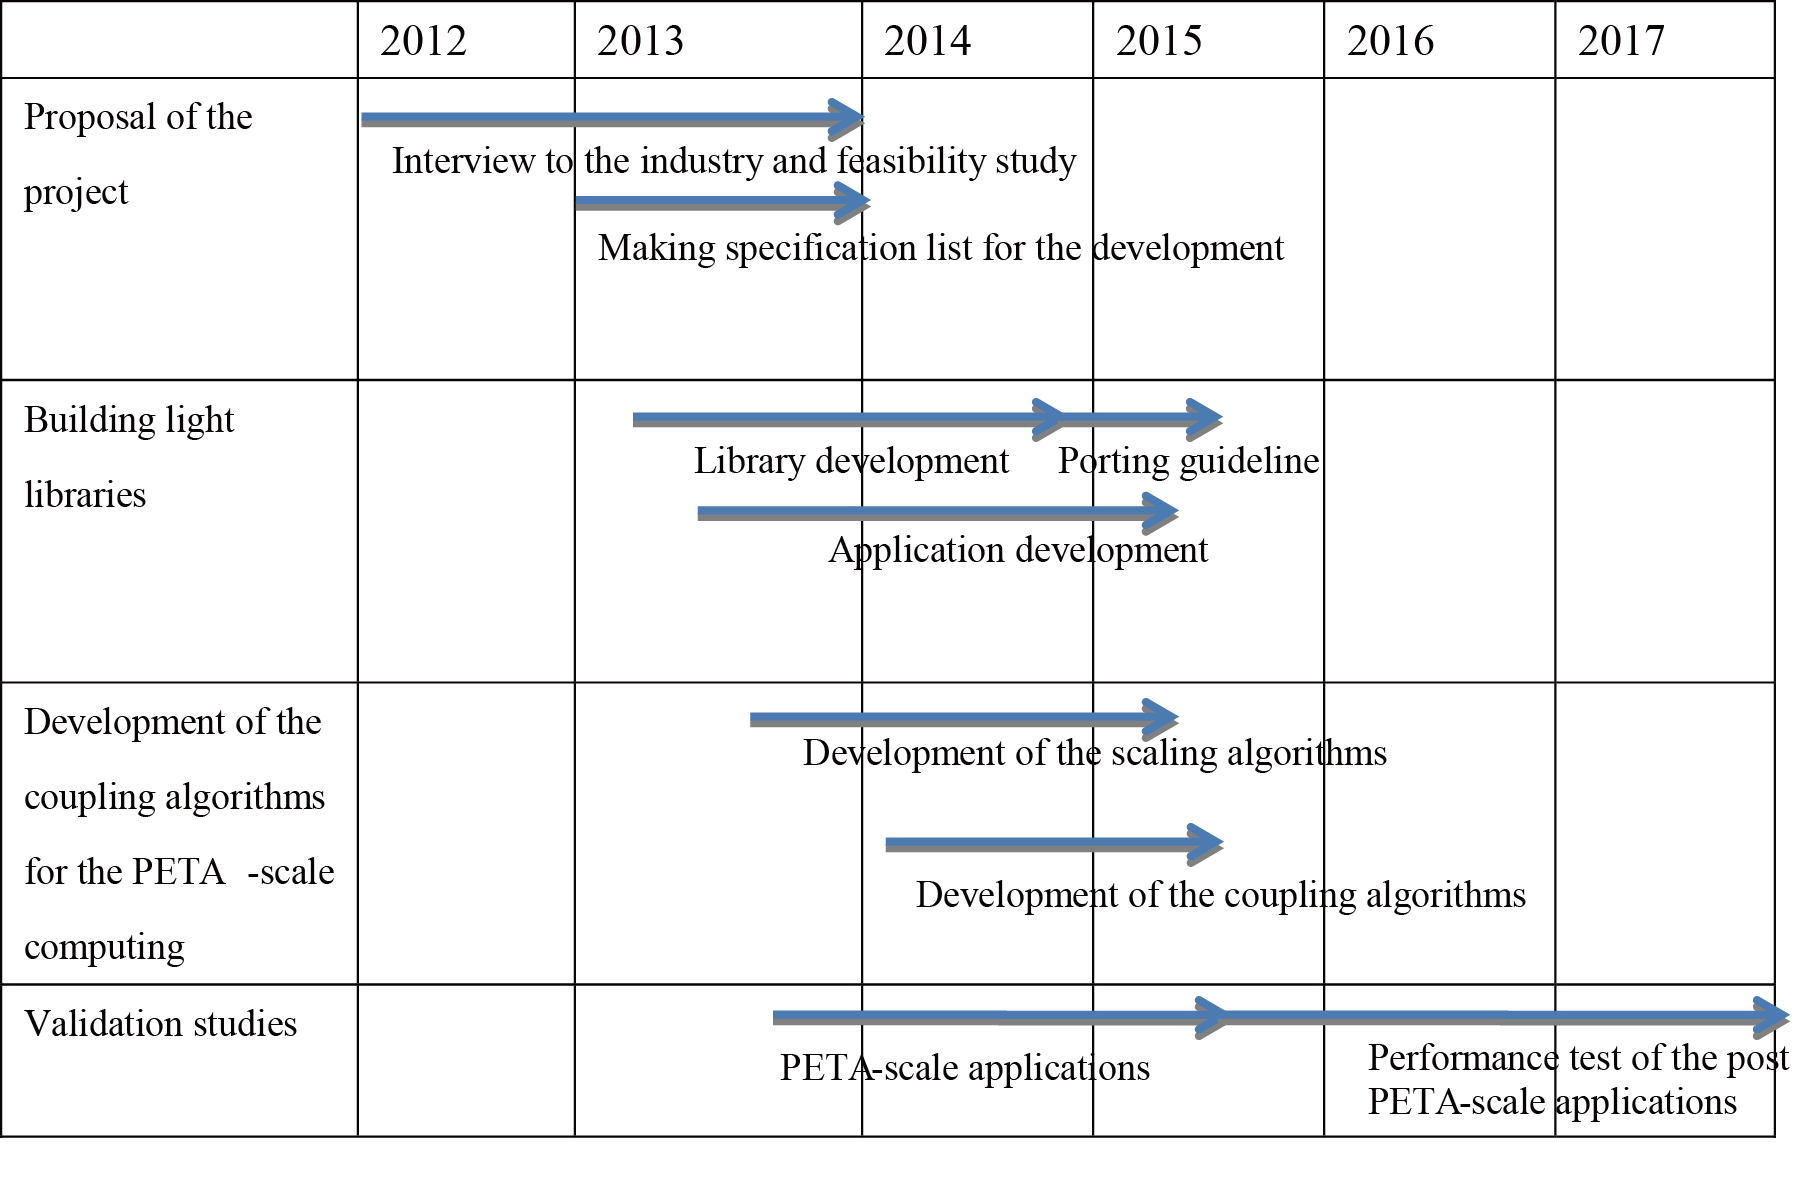
\includegraphics[height=6cm]
  {research/tsubokura/fig11timetable.png}
  \locallabel{fig11}
\end{figure}

%%% DO NOT EDIT BELOW

\section{Publications}

%\printbibliography[keyword=journal, heading=subbibliography, title={Journal Articles}, prefixnumbers={1-}, resetnumbers=true]
%\printbibliography[keyword=proceedings, heading=subbibliography, title={Conference Papers}, prefixnumbers={2-}, resetnumbers=true]
%\printbibliography[keyword=invited, heading=subbibliography, title={Invited Talks}, prefixnumbers={3-}, resetnumbers=true]
%\printbibliography[keyword=poster, heading=subbibliography, title={Posters and Presentations}, prefixnumbers={4-}, resetnumbers=true]
%\printbibliography[keyword=deliverable, heading=subbibliography, title={Patents and Deliverables}, prefixnumbers={5-}, resetnumbers=true]

\printbibliography[keyword=journal, heading=subbibliography, title={Journal Articles}, resetnumbers=true]
\printbibliography[keyword=proceedings, heading=subbibliography, title={Conference Papers}]
\printbibliography[keyword=invited, heading=subbibliography, title={Invited Talks}]
\printbibliography[keyword=poster, heading=subbibliography, title={Posters and Presentations}]
\printbibliography[keyword=deliverable, heading=subbibliography, title={Patents and Deliverables}]

\end{refsection}
